\documentclass[11pt,a4paper]{article}

\usepackage{amsmath,amssymb,amsfonts,amsthm}
\usepackage{hyperref}
\usepackage[round]{natbib}
\usepackage{booktabs}
\usepackage{graphicx}
\usepackage{geometry}
\usepackage{setspace}
\usepackage{float}

\geometry{margin=1in}
\onehalfspacing

\newtheorem{theorem}{Theorem}[section]
\newtheorem{proposition}[theorem]{Proposition}
\newtheorem{lemma}[theorem]{Lemma}
\newtheorem{corollary}[theorem]{Corollary}
\newtheorem{definition}[theorem]{Definition}
\newtheorem{assumption}[theorem]{Assumption}
\newtheorem{remark}[theorem]{Remark}

\hypersetup{
  colorlinks=true,
  linkcolor=blue!60!black,
  citecolor=blue!60!black,
  urlcolor=blue!60!black
}

\title{A Multi-Layer Structural Framework for Bitcoin Treasury Vehicles:\\
Implied Accretion, Leverage Elasticity, and Capital Stack Dynamics}

\author{Haiyang Yu\\
UCLA Anderson School of Management\\
\texttt{haiyang.yu.2026@anderson.ucla.edu}}

\date{March 2026}

\begin{document}
\maketitle

\begin{abstract}
\noindent
We develop a multi-layer stochastic structural model for valuing publicly traded companies whose primary asset is Bitcoin and that employ a leverage flywheel to grow per-share BTC exposure. The canonical example is Strategy (formerly MicroStrategy, MSTR), which as of late 2025 holds over 649{,}000 BTC financed through a complex capital stack of common equity, convertible bonds, and multiple series of perpetual preferred stock. No formal structural framework exists for these ``Bitcoin treasury vehicles,'' leaving investors without rigorous tools to assess whether equity premia reflect achievable BTC accretion or unsustainable leverage.

Our model couples four stochastic processes under the physical measure: (i) BTC price dynamics with jump-diffusion, (ii) an Ornstein--Uhlenbeck process for the equity-over-NAV log-premium capturing market sentiment and mean-reversion, (iii) a compound Poisson process for BTC holding accumulation driven by the leverage flywheel, and (iv) share-count dynamics from equity issuance and convertible conversion. We derive five novel diagnostic indicators---the Implied BTC Growth Rate (IBGR), Implied Leverage Elasticity (ILE), Total Equity Elasticity (TEE), Premium Mean-Reversion Index (PMRI), and Implied Funding Requirement Distribution (IFRD)---that decompose valuation into structural balance-sheet leverage, sentiment premium, and accretion efficiency.

Calibrating to Strategy's publicly available data through December 2025, we find: the model implies an 18.3\% annualized BTC accretion rate (18.4\% per-share), a structural leverage elasticity of 1.17, and a three-year survival probability exceeding 99.4\%. The current premium sits 1.5 standard deviations below its long-run mean, suggesting mean-reversion potential. We extend the framework conceptually to accommodate perpetual preferred stock layers (STRK, STRF) via a priority waterfall, laying groundwork for a complete multi-tranche capital structure analysis.
\end{abstract}


\newpage

\section{Introduction}

\subsection{Motivation}

Strategy (formerly MicroStrategy, ticker MSTR) has become the paradigmatic ``Bitcoin treasury vehicle''---a publicly traded company whose equity value derives overwhelmingly from its Bitcoin holdings rather than operating cash flows. Beginning with an initial 21{,}454 BTC purchase in August 2020, the company has accumulated over 649{,}000 BTC by late 2025, financed through a distinctive flywheel of at-the-market (ATM) equity offerings, convertible bond issuances, and most recently, multiple series of perpetual preferred stock. The resulting capital structure---spanning common equity, convertible debt, and preferred tranches including STRK (8\% convertible preferred), STRF (10\% non-convertible preferred), STRC, STRD, and STRE (EUR-denominated)---has no close precedent in corporate finance.

Strategy's equity has persistently traded at a premium to its net asset value (NAV), with this premium fluctuating dramatically over time. The premium reflects the market's assessment of management's ability to continue acquiring BTC accretively---that is, growing BTC per share even as new shares are issued---combined with the embedded leverage from the debt stack and the optionality of the premium itself. Understanding whether a given premium level is ``justified'' by achievable accretion rates, or whether it reflects unsustainable speculation, is the central question facing investors in MSTR and the growing number of imitators adopting similar strategies.

Despite the significance of this question, no formal structural model exists for Bitcoin treasury vehicles. Traditional corporate structural models in the Merton (1974) tradition treat the firm's assets as following geometric Brownian motion with a fixed capital structure, but Strategy's assets are a single volatile cryptocurrency whose holdings \emph{grow endogenously} in response to the very premium the model seeks to explain. The leverage flywheel creates a feedback loop: a high premium enables equity issuance, which funds BTC purchases, which (if accretive) supports the premium. This circularity demands a purpose-built framework.

\subsection{Research Gap}

The existing literature offers partial tools but no integrated model. Merton's (1974) structural credit model and its extensions (Black and Cox, 1976; Leland, 1994) provide the foundation for modeling equity as a call option on firm assets, but assume exogenous asset dynamics and static capital structures. The growing literature on Bitcoin valuation (Biais et al., 2023; Cong et al., 2021) addresses cryptocurrency pricing but not the corporate wrapper. Convertible bond pricing models (Tsiveriotis and Fernandes, 1998) handle individual instruments but not the full multi-layer stack with endogenous asset accumulation.

The closest practical analogs---closed-end funds trading at premia or discounts to NAV---have been studied extensively (Lee et al., 1991; Pontiff, 1996), but these funds have static portfolios and do not employ leverage flywheels. Strategy's defining feature is that its portfolio is \emph{not} static: the premium drives accumulation, and accumulation supports the premium. This endogeneity is the core modeling challenge we address.

\subsection{Contributions}

This paper makes the following contributions:

\begin{enumerate}
    \item \textbf{A stochastic structural framework for BTC treasury vehicles.} We develop a multi-process model under the physical measure that jointly evolves BTC price, the equity-over-NAV premium, BTC holdings, and share count. The premium follows an Ornstein--Uhlenbeck process capturing mean-reversion, while holdings evolve via a compound Poisson process linked to the flywheel. The model nests several special cases including static treasury, pure-equity financing, and standard Merton-style structural models.

    \item \textbf{Five novel diagnostic indicators.} We derive the Implied BTC Growth Rate (IBGR), which measures the model-implied annualized rate of BTC accumulation both in total and per-share; the Implied Leverage Elasticity (ILE), which decomposes equity sensitivity to BTC into a pure balance-sheet component; the Total Equity Elasticity (TEE), which adds the premium's response to BTC; the Premium Mean-Reversion Index (PMRI), a z-score measuring how far the current premium deviates from its long-run level; and the Implied Funding Requirement Distribution (IFRD), the probability distribution of capital needed to sustain the implied accretion path.

    \item \textbf{Empirical calibration to Strategy.} We calibrate the full model to publicly available data through December 2025, estimating all structural parameters and computing each indicator. The calibration reveals economically interpretable dynamics: an 18.3\% annualized BTC accretion rate, leverage elasticity of 1.17 reflecting moderate balance-sheet leverage, and a premium currently 1.5 stationary standard deviations below its long-run mean. The three-year survival probability exceeds 99.4\%, suggesting the current capital structure is robust to stress.

    \item \textbf{Extension to multi-layer preferred capital stacks.} We outline how the framework extends to accommodate preferred stock layers through a priority waterfall that respects perpetual dividend obligations and conversion optionality, establishing a foundation for full multi-tranche valuation.
\end{enumerate}

\subsection{Paper Outline}

The remainder of the paper is organized as follows. Section~\ref{sec:methodology} presents the structural model: BTC price dynamics, the premium process, holding dynamics, debt and share-count modeling, and the derivation of all five indicators. Section~\ref{sec:results} reports the calibrated parameters and computed indicators with economic interpretation. Section~\ref{sec:discussion} discusses implications for investors, model limitations, and extensions. Section~\ref{sec:conclusion} concludes.


\section{Literature Review}
\label{sec:literature}

This paper draws on several distinct strands of the finance literature.
We synthesize insights from structural credit models, closed-end fund pricing, convertible bond theory, cryptocurrency finance, and capital structure research to build a framework suited to the unique characteristics of Strategy Inc (formerly MicroStrategy) as a BTC-backed equity vehicle.

\subsection{Structural Credit Models}

The foundational framework for linking firm asset values to security prices originates with \citet{merton1974pricing}, who models equity as a European call option on the firm's assets with a strike equal to the face value of debt.
This insight---that limited liability creates option-like payoffs for equity holders---is central to our model's treatment of NAV with a limited liability floor: $\text{NAV}_t = (H_t S_t - D_t)^+$.

\citet{black1976valuing} extend Merton's framework to incorporate safety covenants and subordination, both relevant to Strategy's multi-layered capital structure with preferred stock tranches of differing seniority.
\citet{leland1994corporate} and \citet{leland1996optimal} develop models with endogenous bankruptcy and optimal capital structure, introducing the trade-off between tax shields and distress costs that informs our survival probability analysis.
More recently, \citet{huang2004structural} provide empirical evidence on the performance of structural models, finding that they substantially underpredict credit spreads---the so-called ``credit spread puzzle''---suggesting that factors beyond pure leverage drive credit risk.

In our setting, the single-asset nature of Strategy's balance sheet (essentially only BTC) makes structural models particularly apt: the firm's asset volatility is directly observable via Bitcoin price dynamics, unlike diversified corporations where asset volatility must be inferred.
However, the presence of multiple layers of preferred stock with distinct priority claims extends the standard two-class (debt/equity) Merton framework into a multi-tranche setting analogous to structured credit.

\subsection{NAV Premium and Discount Dynamics}

Strategy trades at a persistent premium to its Bitcoin net asset value, a phenomenon with close parallels to the closed-end fund (CEF) pricing puzzle.
\citet{lee1991investor} propose that investor sentiment drives CEF discounts and premia, with noise trader risk preventing arbitrage from eliminating mispricings.
\citet{pontiff1995closed} documents that CEF premia predict future returns, consistent with mean-reversion---the empirical pattern we capture through our Ornstein--Uhlenbeck premium process $\pi_t$.

\citet{cherkes2009closed} offer a liquidity-based explanation: CEFs provide access to illiquid assets, justifying a premium when the underlying is hard to access directly.
This theory has particular relevance to Strategy, which offers leveraged, operationally-managed BTC exposure that individual investors may find difficult or costly to replicate, especially pre-2024 when spot Bitcoin ETFs were unavailable in the United States.
\citet{dimson1999closed} provide a comprehensive survey of CEF pricing anomalies, noting that premia tend to be larger for funds holding exotic or hard-to-value assets---a characterization that arguably applies to Bitcoin.

The introduction of spot Bitcoin ETFs in January 2024 \citep{alexander2024bitcoin} represents a structural break in the accessibility of BTC exposure, potentially compressing Strategy's premium over time.
Our mean-reverting premium model with regime-dependent long-run mean $\theta$ can accommodate such shifts.
The premium dynamics we observe---with $\pi_t$ positively correlated with BTC returns ($\rho > 0$)---echo the procyclical sentiment patterns documented in the CEF literature.

\subsection{Bitcoin and Cryptocurrency Finance}

The academic literature on Bitcoin pricing has grown rapidly since \citet{nakamoto2008bitcoin}.
\citet{liu2021risks} establish that cryptocurrency returns are driven by network and momentum factors distinct from traditional asset pricing factors, implying that BTC exposure introduces novel risk dimensions to Strategy's equity.
\citet{makarov2020trading} document arbitrage frictions in cryptocurrency markets that can amplify volatility, relevant to our BTC price dynamics specification.

On volatility modeling, \citet{katsiampa2017volatility} compares GARCH specifications for Bitcoin and finds that models with both short- and long-run volatility components best capture BTC dynamics.
\citet{biais2023equilibrium} provide a general equilibrium model of Bitcoin pricing that links fundamentals (mining costs, network adoption) to price, offering theoretical grounding for the drift parameter $\mu_S$ in our $\mathbb{P}$-measure BTC dynamics.
The jump-diffusion specification we employ for BTC prices under $\mathbb{Q}$ follows \citet{merton1976option} and \citet{kou2002jump}, accommodating the well-documented fat tails and discontinuous price movements in cryptocurrency markets \citep{griffin2020bitcoin}.

\subsection{Bitcoin as a Corporate Treasury Asset}

Strategy's pioneering adoption of Bitcoin as a treasury reserve asset, beginning in August 2020, has spawned a small but growing literature.
\citet{vanelli2024bitcoin} study MicroStrategy's treasury strategy and its effects on firm valuation, documenting the reflexive relationship between BTC acquisitions, equity premium, and subsequent capital raises that we formalize as the ``flywheel'' mechanism.
\citet{amin2024corporate} examine more broadly whether corporate cryptocurrency holdings affect firm value, finding heterogeneous effects depending on the scale of holdings relative to firm size.

Our model's BTC holding dynamics---with accumulation rate $\alpha$ driven by the premium $\pi_t^+$ and discrete financing jumps---formalizes the strategic feedback loop whereby a high premium enables accretive capital raises, which increase BTC per share, which supports the premium.
This is a novel contribution: while practitioner analyses have described this flywheel qualitatively, we provide the first stochastic model of its dynamics suitable for Monte Carlo simulation and quantitative indicator extraction.

\subsection{Convertible Bond Pricing and Hybrid Securities}

Strategy's capital structure includes approximately \$8.2 billion in convertible notes alongside five series of preferred stock with varying terms.
The convertible bond pricing literature, beginning with \citet{brennan1977convertible} and \citet{ingersoll1977contingent}, provides the theoretical basis for valuing these hybrid securities.
\citet{tsiveriotis1998valuing} extend the framework to incorporate credit risk, decomposing convertible value into debt and equity components---an approach we use to define ``effective debt'' $D_t^{\text{eff}}$ that adjusts for deep-in-the-money convertibles.
\citet{ammann2003pricing} provide empirical evidence that convertible bonds are systematically underpriced, a finding with implications for the true leverage embedded in Strategy's capital structure.

The preferred stock layer adds further complexity.
\citet{kallberg2013preferred} document that preferred stocks exhibit hybrid risk characteristics, with returns driven by both interest rate and equity market factors.
Strategy's preferred tranches span from pure fixed-income (STRF, STRD) to equity-linked (STRK with conversion into MSTR common), with the variable-rate STRC representing an innovative instrument that adjusts dividends to stabilize price near par---a mechanism without close precedent in the academic literature.

\subsection{Capital Structure and Leverage}

The classical capital structure theories of \citet{modigliani1958cost} and \citet{myers1984capital} provide the backdrop against which Strategy's aggressive leveraging of a single volatile asset must be understood.
\citet{baker2002market} document that firms time equity issuance to exploit high valuations---precisely the behavior we model through premium-dependent financing intensity $\lambda_M(\pi_t)$.

Strategy's capital structure is unusual in several respects that extend standard theory:
(i)~the firm's assets are a single, publicly-traded, highly volatile cryptocurrency;
(ii)~leverage is deliberately and systematically increased to accumulate more of the same asset;
(iii)~the financing flywheel creates a reflexive feedback loop between equity valuation and asset accumulation;
and (iv)~the multi-layered preferred stock structure creates a priority waterfall with complex interactions between dividend obligations, conversion optionality, and residual equity claims.

These features motivate our multi-tranche extension of the Merton framework with endogenous asset accumulation, a contribution at the intersection of structural credit modeling and corporate treasury management.

\subsection{Simulation Methods}

Our quantitative indicators---including the Implied Funding Requirement Distribution (IFRD), per-share Implied BTC Growth Rate (IBGR), and survival probabilities---require Monte Carlo simulation of correlated stochastic processes.
We follow the methods described in \citet{glasserman2004monte}, employing Cholesky decomposition for correlated Brownian motions and thinning algorithms for state-dependent Poisson jump processes.
The Ornstein--Uhlenbeck process for the log-premium follows the exact discretization of \citet{vasicek1977equilibrium}, ensuring that our discrete-time simulation preserves the known transition density of the continuous-time process.


\section{Methodology}
\label{sec:methodology}

This section presents the structural model in full. We begin with the probability space and state variables, then specify each stochastic process, derive the equity valuation identity, and finally define the five diagnostic indicators.

\subsection{Setup: Probability Space and State Variables}

We work on a filtered probability space $(\Omega, \mathcal{F}, (\mathcal{F}_t)_{t \ge 0})$ equipped with two measures:
\begin{itemize}
    \item $\mathbb{P}$: the physical (historical) measure, used for premium dynamics, management behavior (holdings accumulation), survival analysis, and all indicator computations.
    \item $\mathbb{Q}$: the risk-neutral measure, available for calibrating BTC volatility and jump parameters to options data if desired.
\end{itemize}

The model's state variables are:
\begin{itemize}
    \item $S_t$: BTC spot price (BTC-USD).
    \item $H_t$: Strategy's BTC holdings (in BTC).
    \item $D_t$: outstanding debt (face value).
    \item $N_t^{\text{sh}}$: shares of common equity outstanding.
    \item $\pi_t$: log-premium of equity over NAV.
\end{itemize}

From these primitives, we derive:
\begin{align}
    A_t &= H_t S_t, & &\text{(BTC asset value)} \\
    \text{NAV}_t &= (A_t - D_t)^+ = \max(H_t S_t - D_t, 0), & &\text{(net asset value)} \\
    E_t &= P_t N_t^{\text{sh}}, & &\text{(equity market capitalization)} \\
    B_t &= H_t / N_t^{\text{sh}}, & &\text{(BTC per share)}
\end{align}
where $P_t$ is the share price.

To avoid log singularities when computing the historical premium from data, we introduce a floor $\varepsilon > 0$:
\begin{equation}
    \text{NAV}_t^{\text{clip}} = \max(A_t - D_t, \varepsilon),
\end{equation}
and define the log-premium as:
\begin{equation}
    \pi_t = \log\left(\frac{E_t}{\text{NAV}_t^{\text{clip}}}\right).
\end{equation}
Periods where $A_t \approx D_t$ are flagged as a ``distress regime'' and handled separately in calibration.

\subsection{BTC Price Dynamics}

Under the risk-neutral measure $\mathbb{Q}$, for option calibration we consider a jump-diffusion:
\begin{equation}
    \frac{dS_t}{S_{t^-}} = \left(r_t - q_S - \lambda_S k_S\right) dt + \sigma_S(S_t, t)\, dW_t^{S,\mathbb{Q}} + \left(e^{Y_S} - 1\right) dN_t^S,
\end{equation}
where $r_t$ is the risk-free rate, $q_S$ is any BTC carry term (set to zero at baseline), $W_t^{S,\mathbb{Q}}$ is a standard Brownian motion under $\mathbb{Q}$, $N_t^S$ is a Poisson process with intensity $\lambda_S$, $Y_S$ is the log-jump size with distribution $\nu_S$, $k_S = \mathbb{E}[e^{Y_S} - 1]$ is the jump compensator, and $\sigma_S(S_t, t)$ is a potentially state-dependent volatility.

For the physical-measure simulations that drive our indicator computations, we use a simpler geometric Brownian motion calibrated to historical BTC returns:
\begin{equation}
    \frac{dS_t}{S_t} = \mu_S\, dt + \sigma_S\, dW_t^{S,\mathbb{P}},
\end{equation}
with constant drift $\mu_S$ and volatility $\sigma_S$ estimated from daily log-returns.

\subsection{Premium Dynamics}

The log-premium $\pi_t$ is modeled as an Ornstein--Uhlenbeck (OU) process under the physical measure, capturing the empirical observation that premia to NAV exhibit mean-reversion:
\begin{equation}
    d\pi_t = \kappa(\theta - \pi_t)\, dt + \sigma_\pi\, dW_t^{\pi,\mathbb{P}} + \eta_\pi\, dJ_t^\pi,
\end{equation}
where $\kappa > 0$ is the mean-reversion speed, $\theta$ is the long-run mean log-premium, $\sigma_\pi$ is the diffusive volatility, $W_t^{\pi,\mathbb{P}}$ is a Brownian motion under $\mathbb{P}$, and $J_t^\pi$ is an optional pure-jump process with intensity $\lambda_\pi$ (set to zero at baseline).

The BTC and premium Brownian motions are correlated:
\begin{equation}
    \text{corr}(dW_t^{S,\mathbb{P}}, dW_t^{\pi,\mathbb{P}}) = \rho.
\end{equation}

This correlation is economically meaningful: a negative $\rho$ indicates that the premium tends to compress when BTC rises (and vice versa), reflecting a ``buy the rumor, sell the news'' dynamic in NAV-premium relationships.

The exact discrete-time transition for daily step $\Delta t$ is:
\begin{equation}
    \pi_{t+\Delta t} = \theta + (\pi_t - \theta) e^{-\kappa \Delta t} + \sigma_\pi \sqrt{\frac{1 - e^{-2\kappa \Delta t}}{2\kappa}}\, Z_\pi,
\end{equation}
where $(Z_S, Z_\pi)$ are bivariate standard normal with $\text{corr}(Z_S, Z_\pi) = \rho$.

\subsection{BTC Holding Dynamics: The Leverage Flywheel}

The defining feature of a Bitcoin treasury vehicle is that holdings are \emph{endogenous}: management acquires BTC using proceeds from equity and debt issuance, with the pace of acquisition linked to the premium. We model this via:
\begin{equation}
    dH_t = \alpha\, \pi_t^+\, dt + dH_t^{\text{jump}}, \qquad \pi_t^+ = \max(\pi_t, 0),
\end{equation}
where the continuous drift captures routine accumulation scaled by the positive premium, and the jump component captures discrete financing events:
\begin{equation}
    dH_t^{\text{jump}} = \sum_k \Delta H_{\tau_k}\, \delta_{t = \tau_k}, \qquad \Delta H_{\tau_k} \ge 0.
\end{equation}
Here $\{\tau_k\}$ are event times of a Poisson process $M_t$ with intensity $\lambda_M$, and $\Delta H_{\tau_k}$ are BTC amounts purchased. The jump sizes are drawn from an empirical distribution $\mathcal{D}_H$ calibrated to observed purchase events.

In discrete time:
\begin{equation}
    H_{t+\Delta t} = H_t + \alpha \pi_t^+ \Delta t + \sum_{i=1}^{N_t^M} \Delta H_{t,i}, \qquad N_t^M \sim \text{Poisson}(\lambda_M \Delta t).
\end{equation}

When the data suggest $\alpha \approx 0$ (as in our calibration), the model reduces to a pure compound Poisson accumulation process, with all BTC growth occurring through discrete financing events. The intensity or size distribution can be further enriched to depend on leverage or premium levels.

\subsection{Debt and Share-Count Dynamics}

\paragraph{Debt.} At baseline, total outstanding debt is modeled as deterministic and piecewise-constant:
\begin{equation}
    D_t = \sum_{j=1}^J D_j \mathbf{1}_{\{t < T_j\}},
\end{equation}
where each debt instrument $j$ has face value $D_j$ and maturity $T_j$. This conservative treatment ignores the equity-like behavior of deep in-the-money convertibles, providing a solvency lower bound.

\paragraph{Share count.} Shares outstanding evolve through equity issuance and convertible conversion:
\begin{equation}
    dN_t^{\text{sh}} = dN_t^{\text{(equity)}} + dN_t^{\text{(conv)}},
\end{equation}
where both components are jump processes aligned with financing and conversion events. BTC per share is then:
\begin{equation}
    B_t = \frac{H_t}{N_t^{\text{sh}}}.
\end{equation}
The per-share metric $B_t$ is central to assessing whether the flywheel is \emph{accretive}: if $B_t$ grows over time despite share dilution, each share commands more BTC.

\subsection{Equity Valuation Identity}

The structural relation linking equity, assets, debt, and premium is:
\begin{equation}
    E_t = e^{\pi_t} \cdot (H_t S_t - D_t)^+.
    \label{eq:equity_identity}
\end{equation}
This identity holds exactly when $\text{NAV}_t > \varepsilon$ (i.e., outside the distress regime where $\text{NAV}_t^{\text{clip}} = \text{NAV}_t$). It decomposes equity market capitalization into NAV (the intrinsic balance-sheet value) and the exponential of the log-premium (the market's sentiment multiplier). The premium absorbs all factors not captured by current-snapshot NAV: expected future accretion, management optionality, liquidity, and speculative demand.

\subsection{Diagnostic Indicators}

We derive five indicators that together characterize the structural health and valuation of a Bitcoin treasury vehicle.

\subsubsection{Implied BTC Growth Rate (IBGR)}

The total IBGR measures the expected annualized rate of BTC accumulation under the physical measure:
\begin{equation}
    \mu_H = \frac{1}{H_0} \mathbb{E}^{\mathbb{P}} \left[\frac{H_{\Delta t} - H_0}{\Delta t} \;\bigg|\; S_0, \pi_0, H_0 \right] \approx \frac{1}{H_0}\left(\alpha \pi_0^+ + \lambda_M \mathbb{E}[\Delta H]\right).
\end{equation}
The per-share IBGR accounts for dilution:
\begin{equation}
    \mu_{H/N} = \frac{1}{B_0} \mathbb{E}^{\mathbb{P}} \left[\frac{B_{\Delta t} - B_0}{\Delta t} \;\bigg|\; S_0, \pi_0, H_0, N_0^{\text{sh}} \right],
\end{equation}
estimated via Monte Carlo simulation of joint $(H_t, N_t^{\text{sh}})$ paths. Positive $\mu_{H/N}$ indicates accretive growth---the flywheel is delivering more BTC per share despite dilution.

\subsubsection{Implied Leverage Elasticity (ILE)}

The ILE captures the pure balance-sheet sensitivity of equity to BTC price, holding the premium fixed:
\begin{equation}
    \text{ILE}_t = \beta_{LS}(t) = \frac{\partial \log E_t}{\partial \log S_t}\bigg|_{\pi_t\text{ fixed}} = \frac{H_t S_t}{H_t S_t - D_t},
\end{equation}
for $H_t S_t > D_t$. An ILE of 1.17 means a 1\% BTC move produces a 1.17\% equity move from leverage alone, before any premium response.

\subsubsection{Total Equity Elasticity (TEE)}

The TEE incorporates the premium's empirical response to BTC:
\begin{equation}
    \beta_{\text{TOT}}(t) = \frac{d\log E_t}{d\log S_t} = \gamma_{\pi S} + \beta_{LS}(t),
\end{equation}
where $\gamma_{\pi S}$ is the regression coefficient of premium changes on BTC log-returns:
\begin{equation}
    \gamma_{\pi S} \approx \frac{\text{Cov}(\Delta \pi_t, \Delta \log S_t)}{\text{Var}(\Delta \log S_t)}.
\end{equation}
The TEE is what traders experience in their P\&L. When $\gamma_{\pi S} < 0$, premium compression partially offsets leverage, and the TEE may be less than the ILE.

\subsubsection{Premium Mean-Reversion Index (PMRI)}

The PMRI standardizes the current premium against its OU stationary distribution:
\begin{equation}
    \text{PMRI} = \frac{\pi_0 - \theta}{\sigma_\pi / \sqrt{2\kappa}},
\end{equation}
where $\sigma_\pi^2 / (2\kappa)$ is the stationary variance of the OU process. Large positive values signal exuberance; large negative values signal distress or undervaluation.

\subsubsection{Implied Funding Requirement Distribution (IFRD)}

The IFRD characterizes the probability distribution of capital required to sustain the model-implied BTC accumulation trajectory over a horizon $\Delta t$:
\begin{equation}
    G_{\Delta t} = \int_0^{\Delta t} S_u\, dH_u = \int_0^{\Delta t} S_u \alpha \pi_u^+\, du + \sum_{0 < u \le \Delta t} S_u \Delta H_u.
\end{equation}
In discrete simulation:
\begin{equation}
    G_{\Delta t}^{(\text{path})} \approx \sum_{k=0}^{n-1} S_{t_k}(H_{t_{k+1}} - H_{t_k}).
\end{equation}
Monte Carlo over simulated paths provides the empirical distribution of $G_{\Delta t}$, from which we extract the mean, standard deviation, and tail measures (e.g., $\text{VaR}_{95\%}$). Large IFRD values relative to the firm's financing capacity signal potential flywheel unsustainability.

\subsection{Survival and Distress Analysis}

Define a distress event as the first time BTC asset value breaches the debt boundary with buffer $\varepsilon_d \ge 0$:
\begin{equation}
    \tau = \inf\{u \in [0,T] : H_u S_u \le (1+\varepsilon_d) D_u\}.
\end{equation}
The survival probability over horizon $T$ is:
\begin{equation}
    \mathbb{P}(\tau > T) \approx \frac{\#\{\text{paths with no breach before } T\}}{\#\{\text{total simulated paths}\}}.
\end{equation}
This Monte Carlo estimate accounts for the full joint dynamics of BTC price, premium, and holdings accumulation, providing a structurally informed solvency assessment that incorporates the flywheel's stabilizing (or destabilizing) effects.

\subsection{Calibration Strategy}

\paragraph{Premium OU parameters.} Using the exact OU transition density, we estimate $(\kappa, \theta, \sigma_\pi)$ via maximum likelihood on the daily log-premium series, excluding distress-regime observations. The correlation $\rho$ and premium-BTC sensitivity $\gamma_{\pi S}$ are estimated from empirical correlations and OLS regression of premium changes on BTC log-returns.

\paragraph{Holdings dynamics.} We construct the BTC holding change series from public disclosures, identify financing event dates, and estimate jump intensity $\lambda_M$ as the annualized event frequency and mean jump size $\mathbb{E}[\Delta H]$ from the empirical distribution of BTC purchased per event. The continuous drift $\alpha$ is estimated by regressing non-event holding changes on the positive premium; when statistically insignificant (as in our sample), we set $\alpha = 0$.

\paragraph{BTC price parameters.} The drift $\mu_S$ and volatility $\sigma_S$ are estimated from historical daily BTC log-returns under the physical measure.


% theory_endogenous_premium.tex — Endogenous Premium Theory
% Core theoretical contribution: the NAV premium as a perpetual accumulation option

\section{Endogenous Premium Theory}\label{sec:endogenous_premium}

The methodology of Section~\ref{sec:methodology} treats the NAV premium
$\pi_t$ as an exogenous Ornstein--Uhlenbeck process with fixed long-run mean
$\theta$.  This is descriptively adequate but theoretically unsatisfying: it
does not explain \emph{why} a rational market would price a BTC treasury
vehicle above (or below) its net asset value.  This section develops an
endogenous theory of the premium.  The central insight is that the NAV premium
reflects the market value of a \emph{perpetual accumulation option}---the
option to issue equity at a premium and convert proceeds into BTC, thereby
increasing BTC-per-share for existing holders.

We proceed in four parts.  Section~\ref{subsec:endo_system} specifies the
coupled stochastic system that replaces the exogenous OU.
Section~\ref{subsec:fair_premium} derives the equilibrium (fair) premium
$\pi^*$ as the present value of future accretive issuance.
Section~\ref{subsec:reflexivity} characterizes the reflexive feedback loop and
establishes conditions for multiple equilibria.
Section~\ref{subsec:mispricing} defines the mispricing metric and analyzes its
dynamics.

%% ====================================================================
\subsection{The Endogenous Premium System}\label{subsec:endo_system}

\subsubsection{Motivation}

Under the exogenous specification $d\pi_t = \kappa(\theta - \pi_t)\,dt +
\sigma_\pi\,dW_t^\pi$, the long-run mean $\theta$ is a free parameter
estimated from data.  But $\theta$ should itself depend on the firm's
fundamentals: its BTC holdings, leverage, volatility environment, and
capacity to issue accretively.  We now endogenize $\theta$ by replacing it
with a state-dependent equilibrium premium $\pi^*(\Phi_t)$.

\subsubsection{State Vector and Assumptions}

\begin{assumption}[Endogenous Premium Environment]\label{ass:endo_env}
We work under the following conditions:
\begin{enumerate}
  \item The BTC spot price $S_t$ follows geometric Brownian motion under
    $\mathbb{P}$ with drift $\mu_S$ and volatility $\sigma_S$, augmented by
    a market impact term from the firm's BTC purchases.
  \item The firm's BTC holdings $H_t$, debt $D_t$, preferred liabilities
    $P_t^{\mathrm{pfd}}$, and share count $N_t^{\mathrm{sh}}$ evolve as in
    Sections~\ref{sec:methodology}--\ref{sec:model_extended}.
  \item The firm issues equity (ATM) whenever $\pi_t$ exceeds the accretion
    threshold $\pi^*_{\mathrm{ATM}} = \log(\mathrm{ELE}_t)$ from
    Proposition~\ref{prop:accretion}, at a rate proportional to
    $(\pi_t - \pi^*_{\mathrm{ATM}})^+$.
  \item Market participants are risk-neutral (for valuation of the
    accumulation option) and observe the full state vector.
  \item The risk-free rate $r > 0$ is constant.
\end{enumerate}
\end{assumption}

\begin{definition}[State Vector]\label{def:state_vector}
The endogenous premium model is driven by the state vector
\begin{equation}\label{eq:state_vector}
  \Phi_t = \bigl(S_t,\, H_t,\, D_t,\, P_t^{\mathrm{pfd}},\,
  N_t^{\mathrm{sh}},\, \sigma_S,\, \kappa,\, r\bigr),
\end{equation}
from which we derive the ancillary quantities $A_t = H_t S_t$,
$L_t = D_t + P_t^{\mathrm{pfd}}$, $\mathrm{NAV}_t = (A_t - L_t)^+$,
$B_t = H_t / N_t^{\mathrm{sh}}$, and
$\mathrm{ELE}_t = A_t / (A_t - L_t)$.
\end{definition}

\subsubsection{The Coupled SDE System}

\begin{definition}[Endogenous Premium Dynamics]\label{def:endo_sdes}
The endogenous premium model consists of the following coupled system of
stochastic differential equations:
\begin{align}
  \frac{dS_t}{S_t} &= \mu_S\, dt + \sigma_S\, dW_t^S
    + \eta \cdot \frac{dH_t}{H_t},
    \label{eq:dS_endo} \\[6pt]
  d\pi_t &= \kappa\bigl(\pi^*(\Phi_t) - \pi_t\bigr)\, dt
    + \sigma_\pi\, dW_t^\pi,
    \label{eq:dpi_endo} \\[6pt]
  dH_t &= \alpha\, \bigl(\pi_t - \log(\mathrm{ELE}_t)\bigr)^+\, dt
    + dH_t^{\mathrm{jump}},
    \label{eq:dH_endo}
\end{align}
where:
\begin{itemize}
  \item $\eta \ge 0$ is the \emph{market impact coefficient}: each unit of
    BTC purchased by the firm pushes the BTC price by a factor $\eta$.
  \item $\pi^*(\Phi_t)$ is the \emph{equilibrium (fair) premium}, derived
    in Section~\ref{subsec:fair_premium}, replacing the exogenous $\theta$.
  \item $\kappa > 0$ is the mean-reversion speed toward the fair premium.
  \item The accumulation rate in \eqref{eq:dH_endo} is driven by the
    \emph{excess premium} $(\pi_t - \log(\mathrm{ELE}_t))^+$ rather than
    $\pi_t^+$, reflecting that only accretive issuance
    (Proposition~\ref{prop:accretion}) is undertaken.
  \item $\mathrm{corr}(dW_t^S, dW_t^\pi) = \rho$.
\end{itemize}
\end{definition}

\begin{remark}[Comparison with Exogenous Model]\label{rem:comparison}
The exogenous model of Section~\ref{sec:methodology} is recovered by setting
$\eta = 0$ (no market impact), $\pi^*(\Phi_t) = \theta$ (constant long-run
mean), and replacing $(\pi_t - \log(\mathrm{ELE}_t))^+$ with $\pi_t^+$ in
the holding dynamics.  The endogenous model thus nests the exogenous
specification as a special case.
\end{remark}

\begin{remark}[Reflexive Structure]\label{rem:reflexive}
The system \eqref{eq:dS_endo}--\eqref{eq:dH_endo} exhibits Soros-type
reflexivity.  A high premium $\pi_t$ triggers accumulation ($dH_t > 0$),
which via market impact raises $S_t$, which raises $\mathrm{NAV}_t$, which
(if $\pi^*$ increases with fundamentals) raises the fair premium, which
sustains the high observed premium.  The feedback is self-reinforcing in
the upward direction and self-reinforcing in the downward direction, creating
the possibility of multiple equilibria (Section~\ref{subsec:reflexivity}).
\end{remark}

%% ====================================================================
\subsection{Fair Premium Derivation}\label{subsec:fair_premium}

We now derive $\pi^*(\Phi_t)$---the premium that a rational market would
assign to a BTC treasury vehicle given its current fundamentals and
accumulation capacity.

\subsubsection{The Accumulation Option}

\begin{definition}[Accumulation Option]\label{def:accum_option}
The \emph{accumulation option} is the perpetual right to issue equity at a
premium to NAV and convert proceeds into BTC, thereby increasing BTC-per-share.
Its value to existing shareholders at time $t$ is:
\begin{equation}\label{eq:V_accretion}
  V_{\mathrm{acc}}(t) = \mathbb{E}_t\!\left[
    \int_t^\infty e^{-r(u-t)}\,
    \underbrace{\bigl(\pi_u - \log(\mathrm{ELE}_u)\bigr)^+}_{\text{excess premium}}
    \cdot\, \underbrace{q(u)\, S_u}_{\text{BTC value acquired}}
    \cdot\, \underbrace{\frac{N_t^{\mathrm{sh}}}{N_u^{\mathrm{sh}}}
    }_{\text{dilution adjustment}}\,
    du
  \right],
\end{equation}
where $q(u)$ is the rate of BTC acquisition at time $u$ (in BTC per unit time)
and the dilution adjustment accounts for the fact that future issuance dilutes
existing shareholders.
\end{definition}

\begin{remark}
The integral \eqref{eq:V_accretion} has the structure of a perpetual
exchange option: at each instant, the firm can ``exchange'' newly issued
shares (at market price) for BTC (at spot), and the option is in-the-money
whenever the equity premium exceeds the leverage threshold.  The perpetual
nature---there is no expiry on the ATM program---makes this more valuable
than a finite-horizon option.
\end{remark}

\subsubsection{Simplified Closed-Form Derivation}

To obtain a tractable expression for $\pi^*$, we work under a set of
simplifying assumptions.

\begin{assumption}[Stationary Accumulation]\label{ass:stationary}
\begin{enumerate}
  \item The premium $\pi_t$ follows a stationary OU process around $\pi^*$
    with speed $\kappa$ and volatility $\sigma_\pi$.
  \item BTC holdings grow at a constant proportional rate $g_H$ (the
    model-implied IBGR from Section~\ref{sec:methodology}).
  \item Dilution offsets a fraction $\delta$ of gross BTC growth, so the
    net per-share BTC growth rate is $g_B = g_H - \delta$.
  \item The leverage ratio $\ell_t = L_t / A_t$ is approximately constant
    at $\bar{\ell}$.
  \item Market impact is small: $\eta \ll 1$.
\end{enumerate}
\end{assumption}

\begin{proposition}[Accretive Issuance Value]\label{prop:accretion_value}
Under Assumptions~\ref{ass:endo_env} and~\ref{ass:stationary}, the
per-share value of the accumulation option is
\begin{equation}\label{eq:V_acc_closed}
  V_{\mathrm{acc}} = \mathrm{NAV}_t^{\mathrm{ps}} \cdot
  \frac{g_B}{r - g_B} \cdot
  \Psi(\pi^*, \kappa, \sigma_\pi, \bar{\ell}),
\end{equation}
where $\mathrm{NAV}_t^{\mathrm{ps}} = \mathrm{NAV}_t / N_t^{\mathrm{sh}}$
is per-share NAV, $g_B$ is the net per-share BTC growth rate, and
\begin{equation}\label{eq:Psi}
  \Psi(\pi^*, \kappa, \sigma_\pi, \bar\ell) =
  \Phi_{\mathrm{N}}\!\left(
    \frac{\pi^* - \log(1/(1-\bar\ell))}{\sigma_\pi / \sqrt{2\kappa}}
  \right)
  \cdot \left(1 + \frac{\sigma_\pi^2}{4\kappa\, r}\right)
\end{equation}
is the \emph{accumulation efficiency factor}.  Here
$\Phi_{\mathrm{N}}(\cdot)$ is the standard normal CDF.
\end{proposition}

\begin{proof}
Under Assumption~\ref{ass:stationary}, the premium fluctuates around $\pi^*$
with stationary distribution
$\pi \sim \mathcal{N}(\pi^*,\, \sigma_\pi^2 / (2\kappa))$.  The accumulation
option is exercised whenever $\pi_t > \log(\mathrm{ELE}_t) =
\log(1/(1-\bar\ell))$.  The probability that the option is in-the-money at
any given time is
\begin{equation}\label{eq:prob_itm}
  p_{\mathrm{ITM}} = \mathbb{P}\!\left(
    \pi_t > \log\!\left(\frac{1}{1-\bar\ell}\right)
  \right)
  = \Phi_{\mathrm{N}}\!\left(
    \frac{\pi^* - \log(1/(1-\bar\ell))}{\sigma_\pi / \sqrt{2\kappa}}
  \right).
\end{equation}

When in-the-money, the expected excess premium is proportional to
$\sigma_\pi / \sqrt{2\kappa}$ (the standard deviation of the stationary
distribution), contributing the correction factor $(1 + \sigma_\pi^2 /
(4\kappa r))$ after integrating the discounted expected payoff.

The per-share value of BTC accretion is a perpetuity growing at rate $g_B$,
discounted at rate $r$:
\[
  \mathrm{NAV}_t^{\mathrm{ps}} \cdot \frac{g_B}{r - g_B}
\]
whenever $g_B < r$ (transversality condition).  Multiplying by the fraction
of time the option is exercisable and the volatility correction yields
\eqref{eq:V_acc_closed}.
\end{proof}

\subsubsection{The Fair Premium}

\begin{theorem}[Fair Premium]\label{thm:fair_premium}
Under Assumptions~\ref{ass:endo_env} and~\ref{ass:stationary}, the
equilibrium log-premium $\pi^*$ satisfies the fixed-point equation
\begin{equation}\label{eq:pi_star_fp}
  \boxed{
    \pi^* = \log\!\left(1 + \frac{V_{\mathrm{acc}}}{\mathrm{NAV}_t^{\mathrm{ps}}}\right)
    = \log\!\left(1 + \frac{g_B}{r - g_B}\,
    \Psi(\pi^*, \kappa, \sigma_\pi, \bar\ell)\right).
  }
\end{equation}
\end{theorem}

\begin{proof}
The equity market capitalization per share equals NAV per share plus the
value of the accumulation option:
\begin{equation}\label{eq:equity_decomp_endo}
  \frac{E_t}{N_t^{\mathrm{sh}}}
  = \mathrm{NAV}_t^{\mathrm{ps}} + V_{\mathrm{acc}}.
\end{equation}
The log-premium is $\pi_t = \log(E_t / \mathrm{NAV}_t)$, so in equilibrium:
\begin{align}
  e^{\pi^*} &= \frac{E_t / N_t^{\mathrm{sh}}}{\mathrm{NAV}_t / N_t^{\mathrm{sh}}}
  = \frac{\mathrm{NAV}_t^{\mathrm{ps}} + V_{\mathrm{acc}}}
         {\mathrm{NAV}_t^{\mathrm{ps}}}
  = 1 + \frac{V_{\mathrm{acc}}}{\mathrm{NAV}_t^{\mathrm{ps}}}.
  \label{eq:pi_star_derivation}
\end{align}
Substituting \eqref{eq:V_acc_closed} and taking logarithms yields
\eqref{eq:pi_star_fp}.

This is a fixed-point equation because $\Psi$ depends on $\pi^*$ through
the normal CDF term in \eqref{eq:Psi}.  Existence and uniqueness are
established in Proposition~\ref{prop:fp_existence}.
\end{proof}

\begin{proposition}[Existence and Uniqueness of Fair Premium]%
\label{prop:fp_existence}
Define the map
$F(\pi) = \log\!\bigl(1 + (g_B/(r-g_B))\,\Psi(\pi, \kappa, \sigma_\pi,
\bar\ell)\bigr)$.  Under the condition $g_B < r$:
\begin{enumerate}
  \item $F$ maps $\mathbb{R}$ into $[0, \bar\pi]$ where
    $\bar\pi = \log(1 + g_B/(r-g_B)) < \infty$.
  \item $F$ is increasing and Lipschitz with constant
    $\mathrm{Lip}(F) < 1$ whenever
    \begin{equation}\label{eq:contraction_cond}
      \frac{g_B}{r - g_B} \cdot
      \frac{\phi_{\mathrm{N}}(\cdot)}{\sigma_\pi / \sqrt{2\kappa}}
      \cdot \frac{1}{1 + g_B \Psi / (r - g_B)} < 1,
    \end{equation}
    where $\phi_{\mathrm{N}}$ is the standard normal PDF.
  \item Under \eqref{eq:contraction_cond}, $F$ is a contraction mapping on
    $[0, \bar\pi]$, so by the Banach fixed-point theorem there exists a
    unique $\pi^* \in [0, \bar\pi]$ satisfying $F(\pi^*) = \pi^*$.
\end{enumerate}
\end{proposition}

\begin{proof}
\emph{(i)} Since $\Psi \in [0, 1 + \sigma_\pi^2/(4\kappa r)]$ and
$g_B/(r-g_B) > 0$, we have $F(\pi) \in [0, \bar\pi]$ for all $\pi$.

\emph{(ii)} The derivative of $F$ is
\[
  F'(\pi) = \frac{g_B/(r-g_B)}{1 + g_B\,\Psi(\pi)/(r-g_B)}
  \cdot \frac{\partial \Psi}{\partial \pi}.
\]
Since $\partial\Psi/\partial\pi = \phi_{\mathrm{N}}(\cdot) /
(\sigma_\pi/\sqrt{2\kappa}) \cdot (1 + \sigma_\pi^2/(4\kappa r))$, the
Lipschitz constant is bounded by the supremum of $|F'|$, which is finite.
Condition \eqref{eq:contraction_cond} ensures $\sup|F'| < 1$.

\emph{(iii)} A contraction mapping on a complete metric space (the closed
interval $[0,\bar\pi] \subset \mathbb{R}$) has a unique fixed point by
the Banach theorem.
\end{proof}

\subsubsection{Comparative Statics}

\begin{proposition}[Comparative Statics of the Fair Premium]%
\label{prop:comp_statics}
The equilibrium premium $\pi^*$ satisfies the following comparative statics:
\begin{align}
  \frac{\partial \pi^*}{\partial g_B} &> 0
    &\quad& \text{(higher per-share BTC growth $\Rightarrow$ higher premium)},
    \label{eq:cs_gB} \\[4pt]
  \frac{\partial \pi^*}{\partial \sigma_S} &> 0
    &\quad& \text{(higher BTC volatility $\Rightarrow$ higher premium)},
    \label{eq:cs_sigma} \\[4pt]
  \frac{\partial \pi^*}{\partial \kappa} &< 0
    &\quad& \text{(faster mean-reversion $\Rightarrow$ lower premium)},
    \label{eq:cs_kappa} \\[4pt]
  \frac{\partial \pi^*}{\partial \bar\ell} &\lessgtr 0
    &\quad& \text{(leverage: non-monotone)},
    \label{eq:cs_ell} \\[4pt]
  \frac{\partial \pi^*}{\partial r} &< 0
    &\quad& \text{(higher discount rate $\Rightarrow$ lower premium)}.
    \label{eq:cs_r}
\end{align}
\end{proposition}

\begin{proof}
We apply the implicit function theorem to $G(\pi^*, \theta) =
\pi^* - F(\pi^*; \theta) = 0$, where $\theta$ denotes a generic parameter.
Since $\partial G / \partial \pi^* = 1 - F'(\pi^*) > 0$ by the contraction
condition, we have
\begin{equation}\label{eq:ift}
  \frac{\partial \pi^*}{\partial \theta}
  = \frac{\partial F / \partial \theta}{1 - F'(\pi^*)}.
\end{equation}
The sign is determined by $\partial F / \partial \theta$:

\emph{BTC growth rate $g_B$:} $\partial F / \partial g_B > 0$ since
higher growth increases both $g_B/(r-g_B)$ and the present value of future
accretion.

\emph{BTC volatility $\sigma_S$:} Higher $\sigma_S$ increases BTC price
dispersion, which increases the expected future NAV growth (via the convexity
of the equity claim on BTC) and raises the value of the accumulation option.
This effect operates through $g_B$, which is increasing in $\sigma_S$ via
the flywheel's option-like payoff.

\emph{Mean-reversion speed $\kappa$:} Higher $\kappa$ reduces the
stationary variance $\sigma_\pi^2/(2\kappa)$ of the premium, making extreme
premium excursions (which drive the most accretive issuance) less likely.
This lowers $\Psi$ and hence $\pi^*$.

\emph{Leverage $\bar\ell$:} The effect is non-monotone.  Higher leverage
raises the accretion threshold $\log(1/(1-\bar\ell))$, reducing the
probability that issuance is accretive (lowering $p_{\mathrm{ITM}}$).
However, higher leverage also amplifies BTC returns via $\mathrm{ELE}_t$,
potentially increasing $g_B$.  At low leverage, the amplification effect
dominates; at high leverage, the threshold effect dominates, creating an
interior optimum.

\emph{Discount rate $r$:} Higher $r$ reduces the present value of the
perpetuity $g_B/(r-g_B)$, directly lowering $\pi^*$.
\end{proof}

\begin{remark}[Volatility as Value Driver]\label{rem:vol_value}
The comparative static $\partial\pi^*/\partial\sigma_S > 0$ is one of the
model's most distinctive predictions: unlike a standard equity, where higher
volatility increases risk and reduces value (all else equal), a BTC treasury
vehicle \emph{benefits} from higher BTC volatility because it makes the
accumulation option more valuable.  This is analogous to the vega of a call
option.  Empirically, MSTR's premium has tended to expand during periods of
elevated BTC volatility, consistent with this prediction.
\end{remark}

\subsubsection{Conditions for Premium vs.\ Discount}

\begin{proposition}[Premium--Discount Boundary]\label{prop:premium_discount}
The fair premium satisfies $\pi^* > 0$ (premium to NAV) if and only if the
accumulation option has positive value, which requires:
\begin{equation}\label{eq:premium_condition}
  g_B > 0
  \quad\text{and}\quad
  p_{\mathrm{ITM}} > 0
  \quad\text{and}\quad
  g_B < r.
\end{equation}
The fair premium satisfies $\pi^* < 0$ (discount to NAV) when either:
\begin{enumerate}
  \item $g_B < 0$: dilution exceeds gross BTC accumulation, destroying
    per-share value; or
  \item The firm faces a perpetual cash drain (preferred dividends, debt
    coupons) that exceeds expected asset appreciation, so the ongoing
    liabilities reduce NAV faster than the flywheel builds it.
\end{enumerate}
\end{proposition}

\begin{proof}
From \eqref{eq:pi_star_fp}, $\pi^* > 0$ iff
$V_{\mathrm{acc}} / \mathrm{NAV}_t^{\mathrm{ps}} > 0$.  By
\eqref{eq:V_acc_closed}, $V_{\mathrm{acc}} > 0$ requires $g_B > 0$
(positive net accretion), $\Psi > 0$ (positive probability of accretive
issuance), and $r > g_B$ (finite present value).  All three conditions
in \eqref{eq:premium_condition} are necessary and sufficient.

For the discount case, when the firm faces perpetual liabilities with
present value exceeding the accumulation option, we extend
\eqref{eq:equity_decomp_endo} to
\[
  \frac{E_t}{N_t^{\mathrm{sh}}}
  = \mathrm{NAV}_t^{\mathrm{ps}} + V_{\mathrm{acc}}
  - \mathrm{PV}(\text{net liability drag}),
\]
where the net liability drag is the present value of preferred dividends
and coupons net of expected asset appreciation from the flywheel.
When $V_{\mathrm{acc}} < \mathrm{PV}(\text{drag})$, the premium turns
negative.
\end{proof}

\begin{remark}[Interpreting NAV Discounts]
A persistent NAV discount ($\pi^* < 0$) signals that the market views the
firm's capital structure as value-destroying: the cost of servicing
liabilities exceeds the benefit of the accumulation option.  This can occur
when (i) the premium is too low for accretive ATM issuance, (ii) convertible
debt conversion dilutes without commensurate BTC growth, or (iii) preferred
dividend obligations ($\Phi_t$) consume expected returns.  The discount is
\emph{rational} in this framework, not a market inefficiency.
\end{remark}

%% ====================================================================
\subsection{Reflexivity and Multiple Equilibria}\label{subsec:reflexivity}

The coupled system \eqref{eq:dS_endo}--\eqref{eq:dH_endo} exhibits
self-reinforcing dynamics that can generate multiple equilibria.  We now
formalize this mechanism.

\subsubsection{The Feedback Map}

\begin{definition}[Feedback Map]\label{def:feedback_map}
Define the \emph{premium feedback map}
$\mathcal{F}: \pi \mapsto \pi'$ as the composition of:
\begin{enumerate}
  \item \textbf{Accumulation:} Premium $\pi$ induces BTC acquisition at
    rate $q(\pi) = \alpha(\pi - \log(\mathrm{ELE}))^+$.
  \item \textbf{Market impact:} BTC purchases push the BTC price by
    $\Delta S / S = \eta \cdot q(\pi) / H$.
  \item \textbf{NAV update:} Higher $S$ raises $\mathrm{NAV}$ and
    potentially changes the fair premium.
  \item \textbf{Premium update:} The market re-prices the accumulation
    option given the updated state, yielding $\pi' = \pi^*(\Phi')$.
\end{enumerate}
An equilibrium is a fixed point of $\mathcal{F}$: $\pi = \mathcal{F}(\pi)$.
\end{definition}

\begin{theorem}[Multiple Equilibria]\label{thm:multiple_eq}
Under Assumptions~\ref{ass:endo_env}--\ref{ass:stationary}, if the market
impact parameter $\eta$ is sufficiently large and the accumulation rate
$\alpha$ is sufficiently responsive to the premium, there exist (generically)
three equilibria:
\begin{enumerate}
  \item \textbf{High-premium equilibrium} $\pi_H^* > 0$: The premium is
    high, the firm issues accretively, BTC accumulation supports the BTC
    price, and the premium is self-sustaining.  This equilibrium is
    \emph{locally stable}.
  \item \textbf{Low-premium (discount) equilibrium} $\pi_L^* \le 0$: The
    premium is at or below zero, the firm cannot issue accretively, there is
    no BTC accumulation, no market impact support, and the discount is
    self-reinforcing.  This equilibrium is \emph{locally stable}.
  \item \textbf{Unstable equilibrium} $\pi_U^* \in (\pi_L^*, \pi_H^*)$:
    An intermediate premium that is a saddle point---any perturbation pushes
    the system toward either $\pi_H^*$ or $\pi_L^*$.
\end{enumerate}
\end{theorem}

\begin{proof}
Consider the net premium adjustment function
$G(\pi) = \mathcal{F}(\pi) - \pi$, which measures the difference between
the implied fair premium and the current premium.  An equilibrium satisfies
$G(\pi) = 0$.

\emph{Step 1: Shape of $G$.}
At $\pi \to -\infty$, no issuance occurs, so $q(\pi) = 0$, there is no
market impact, and the fair premium is determined solely by the (negative)
liability drag: $\mathcal{F}(\pi) = \pi_0^{\mathrm{base}} > -\infty$, a
finite value.  Thus $G(\pi) > 0$ for sufficiently negative $\pi$.

At $\pi \to +\infty$, issuance is massive, but per-share dilution grows
proportionally, and the marginal value of additional BTC decreases (each
additional BTC is purchased at an increasingly high dollar cost due to
market impact).  Thus $\mathcal{F}(\pi)$ grows slower than $\pi$, and
$G(\pi) < 0$ for sufficiently large $\pi$.

\emph{Step 2: Non-monotonicity.}
For intermediate $\pi$, the feedback loop creates a region where
$\mathcal{F}(\pi)$ exceeds $\pi$: the market impact of accumulation raises
the BTC price, which raises NAV, which raises the fair premium above the
current premium.  Specifically, when the premium crosses the accretion
threshold $\log(\mathrm{ELE})$ from below, the accumulation option
``switches on,'' creating a discrete increase in $\mathcal{F}$.

Combined with the concavity of $\mathcal{F}$ at high $\pi$ (diminishing
returns) and the flat region at low $\pi$ (no issuance), $G$ crosses zero
three times, yielding three fixed points.

\emph{Step 3: Stability.}
At $\pi_H^*$: $\mathcal{F}'(\pi_H^*) < 1$, so the equilibrium is stable
(perturbations are dampened by the mean-reversion of $\pi_t$).

At $\pi_L^*$: $\mathcal{F}'(\pi_L^*) < 1$ (the system is in the flat
region with no feedback), so this equilibrium is also stable.

At $\pi_U^*$: $\mathcal{F}'(\pi_U^*) > 1$ (the feedback amplifies
perturbations), making this equilibrium unstable.
\end{proof}

\subsubsection{Characterization of Equilibria}

\begin{proposition}[High-Premium Equilibrium]\label{prop:high_eq}
The high-premium equilibrium $\pi_H^*$ satisfies
\begin{equation}\label{eq:pi_H}
  \pi_H^* \approx \log\!\left(1 + \frac{g_B + \eta\, q_H / H}{r - g_B}
  \right),
\end{equation}
where $q_H = \alpha(\pi_H^* - \log(\mathrm{ELE}))^+$ is the equilibrium
accumulation rate.  The premium is sustained by:
\begin{enumerate}
  \item Accretive issuance (positive $g_B$), which grows BTC per share.
  \item Market impact ($\eta q_H / H$), which supports BTC price.
  \item Self-fulfilling expectations: the premium enables the issuance
    that justifies the premium.
\end{enumerate}
\end{proposition}

\begin{proof}
Substitute the market-impact-augmented BTC growth rate $\tilde{g}_B =
g_B + \eta q_H / H$ into the fair premium formula
\eqref{eq:pi_star_fp}.  The market impact term increases the effective
growth rate, which raises the present value of the accumulation option and
hence the premium.  The equilibrium is self-consistent because $q_H$ itself
depends on $\pi_H^*$.
\end{proof}

\begin{proposition}[Death Spiral Equilibrium]\label{prop:death_spiral}
The low-premium equilibrium $\pi_L^*$ is characterized by:
\begin{equation}\label{eq:pi_L}
  \pi_L^* \approx -\frac{\mathrm{PV}(\text{liability drag})}
  {\mathrm{NAV}_t^{\mathrm{ps}}},
\end{equation}
where the liability drag includes preferred dividend obligations $\Phi_t$
and coupon payments net of any residual operating cash flows.  The death
spiral mechanism operates as follows:
\begin{enumerate}
  \item Low premium $\pi_t < \log(\mathrm{ELE}_t)$ $\Rightarrow$
    no accretive ATM issuance possible.
  \item No accumulation $\Rightarrow$ no market impact support for $S_t$.
  \item BTC price stagnation or decline $\Rightarrow$ NAV falls.
  \item Ongoing liability payments (dividends, coupons) drain assets
    $\Rightarrow$ NAV falls further.
  \item Leverage $\ell_t$ rises $\Rightarrow$ accretion threshold
    $\log(1/(1-\ell_t))$ rises $\Rightarrow$ even harder to issue
    accretively.
  \item If the firm issues non-accretive preferred (last resort per
    Theorem~\ref{thm:optimal_channel}), $\Phi_t$ increases, adding
    more liability drag.
\end{enumerate}
\end{proposition}

\begin{proof}
When $\pi_t < \log(\mathrm{ELE}_t)$, the accumulation option value
$V_{\mathrm{acc}} = 0$ (the option is out-of-the-money with zero
probability of exercise under the stationary distribution).  The equity
value then equals NAV minus the present value of net liabilities:
\[
  E_t = \mathrm{NAV}_t - \mathrm{PV}(\text{liability drag}),
\]
so $\pi_L^* = \log(E_t / \mathrm{NAV}_t) < 0$ when the drag is positive.
Each step in the spiral raises $\ell_t$ or $\Phi_t$, increasing the drag
and deepening the discount, confirming local stability.
\end{proof}

\subsubsection{The Tipping Point}

\begin{definition}[Critical Premium]\label{def:critical_premium}
The \emph{critical premium} $\pi_c$ is the unstable equilibrium $\pi_U^*$
that separates the basins of attraction of the high-premium and death-spiral
equilibria:
\begin{equation}\label{eq:pi_critical}
  \pi_c = \pi_U^* = \inf\bigl\{\pi > \pi_L^* : G(\pi) = 0,\;
  G'(\pi) > 0 \bigr\}.
\end{equation}
\end{definition}

\begin{proposition}[Tipping Point Characterization]\label{prop:tipping}
The critical premium satisfies
\begin{equation}\label{eq:tipping_approx}
  \pi_c \approx \log(\mathrm{ELE}_t)
  + \frac{\sigma_\pi}{\sqrt{2\kappa}} \cdot
  \Phi_{\mathrm{N}}^{-1}\!\left(
    \frac{r - g_B}{g_B} \cdot \frac{e^{\pi_c} - 1}{1 + \sigma_\pi^2/(4\kappa r)}
  \right),
\end{equation}
and is approximately equal to the accretion threshold
$\log(\mathrm{ELE}_t)$ when market impact $\eta$ is small.
The tipping point has the following sensitivities:
\begin{align}
  \frac{\partial \pi_c}{\partial \bar\ell} &> 0
    &\quad& \text{(higher leverage raises the tipping point)},
    \label{eq:tip_ell} \\
  \frac{\partial \pi_c}{\partial \Phi_t} &> 0
    &\quad& \text{(higher dividend burden raises the tipping point)},
    \label{eq:tip_phi} \\
  \frac{\partial \pi_c}{\partial \sigma_S} &< 0
    &\quad& \text{(higher BTC vol lowers the tipping point)}.
    \label{eq:tip_sigma}
\end{align}
\end{proposition}

\begin{proof}
The tipping point is the premium at which the accumulation option value
just offsets the liability drag.  At $\pi_c$, the marginal value of a small
premium increase (which enables some accretive issuance) exactly equals the
marginal cost (the liability drag per unit time).  Setting
$V_{\mathrm{acc}}(\pi_c) = \mathrm{PV}(\text{drag})$ and solving for
$\pi_c$ using \eqref{eq:V_acc_closed} yields \eqref{eq:tipping_approx}.

The comparative statics follow from the implicit function theorem applied
to $G(\pi_c; \theta) = 0$:
\begin{itemize}
  \item Higher $\bar\ell$ raises $\log(\mathrm{ELE})$, requiring a higher
    premium to reach the accretive region.
  \item Higher $\Phi_t$ increases the liability drag that the accumulation
    option must offset.
  \item Higher $\sigma_S$ increases the option value for any given premium,
    lowering the premium needed to break even.  \qedhere
\end{itemize}
\end{proof}

\begin{remark}[Policy Implication]
The tipping point $\pi_c$ is the most important quantity for risk management.
Management should monitor the distance $\pi_t - \pi_c$: when this is large
and positive, the firm is safely in the high-premium basin.  When it
approaches zero, the firm is at risk of transitioning to the death spiral.
Issuing non-convertible preferred stock (which raises both $\bar\ell$ and
$\Phi_t$) pushes $\pi_c$ upward, shrinking the safety margin---a prediction
consistent with market reactions to STRF issuance.
\end{remark}

\subsubsection{Phase Diagram}

\begin{proposition}[Phase Diagram in $(\pi, S)$ Space]\label{prop:phase}
The dynamics of the endogenous premium system can be summarized in a
phase diagram with two regions separated by the critical surface
$\pi = \pi_c(\Phi_t)$:
\begin{enumerate}
  \item \textbf{Virtuous cycle region} ($\pi_t > \pi_c$):
    The drift of $\pi_t$ is toward $\pi_H^*$ from below, and the BTC price
    receives positive support from accumulation.  The expected trajectory is
    toward the high-premium equilibrium.
  \item \textbf{Death spiral region} ($\pi_t < \pi_c$):
    The drift of $\pi_t$ is toward $\pi_L^*$ from above, and BTC receives
    no accumulation support.  The expected trajectory is toward the discount
    equilibrium, with the approach accelerating as leverage rises.
\end{enumerate}
The velocity of the dynamics is:
\begin{equation}\label{eq:drift_pi}
  \mathbb{E}[d\pi_t \mid \pi_t = \pi] =
  \begin{cases}
    \kappa(\pi_H^* - \pi)\,dt & \text{if } \pi > \pi_c, \\[4pt]
    \kappa(\pi_L^* - \pi)\,dt & \text{if } \pi < \pi_c.
  \end{cases}
\end{equation}
\end{proposition}

\begin{proof}
This follows directly from the definition of $\pi_c$ as the boundary between
basins of attraction.  In each region, the premium mean-reverts toward the
locally stable equilibrium at speed $\kappa$.  At $\pi = \pi_c$ the drift
is zero (the unstable equilibrium), and any perturbation determines the
direction of subsequent evolution.
\end{proof}

%% ====================================================================
\subsection{Mispricing Dynamics}\label{subsec:mispricing}

We now define the deviation of the observed premium from its fair value and
characterize its dynamics.

\begin{definition}[Mispricing]\label{def:mispricing}
The \emph{mispricing} at time $t$ is the difference between the observed
log-premium and the fair log-premium:
\begin{equation}\label{eq:delta_def}
  \Delta_t = \pi_t - \pi^*(\Phi_t).
\end{equation}
Positive $\Delta_t$ indicates overvaluation (the market assigns a higher
premium than fundamentals justify).  Negative $\Delta_t$ indicates
undervaluation.
\end{definition}

\begin{theorem}[Mispricing Dynamics]\label{thm:mispricing_dynamics}
Under the endogenous premium system
\eqref{eq:dS_endo}--\eqref{eq:dH_endo}, the mispricing $\Delta_t$ follows
\begin{equation}\label{eq:d_delta}
  d\Delta_t = -\kappa_\Delta\, \Delta_t\, dt
  + \sigma_\Delta\, d\tilde{W}_t,
\end{equation}
where
\begin{align}
  \kappa_\Delta &= \kappa + \frac{\partial \pi^*}{\partial \Phi}
    \cdot \frac{\partial \Phi}{\partial \pi}\bigg|_{\pi = \pi^*}
    > \kappa,
    \label{eq:kappa_delta} \\[4pt]
  \sigma_\Delta^2 &= \sigma_\pi^2
    + \left(\frac{\partial \pi^*}{\partial S}\right)^2 \sigma_S^2 S_t^2
    - 2\rho\, \sigma_\pi \cdot \frac{\partial \pi^*}{\partial S}\,
    \sigma_S S_t,
    \label{eq:sigma_delta}
\end{align}
and $\tilde{W}_t$ is a Brownian motion under $\mathbb{P}$.  The key result
is that $\kappa_\Delta > \kappa$: \emph{mispricing mean-reverts faster than
the premium itself}.
\end{theorem}

\begin{proof}
Apply It\^{o}'s lemma to $\Delta_t = \pi_t - \pi^*(\Phi_t)$:
\begin{equation}\label{eq:ito_delta}
  d\Delta_t = d\pi_t - d\pi^*(\Phi_t).
\end{equation}
The first term is given by \eqref{eq:dpi_endo}:
\[
  d\pi_t = \kappa(\pi^* - \pi_t)\,dt + \sigma_\pi\,dW_t^\pi
  = -\kappa\,\Delta_t\,dt + \sigma_\pi\,dW_t^\pi.
\]
For the second term, $\pi^*$ depends on $\Phi_t$ which evolves with
$S_t$ and $H_t$.  By the chain rule:
\[
  d\pi^* = \frac{\partial \pi^*}{\partial S}\,dS_t
  + \frac{\partial \pi^*}{\partial H}\,dH_t + \cdots
\]
The crucial feedback term is $(\partial\pi^*/\partial\Phi) \cdot
(\partial\Phi/\partial\pi)$: when the premium is above $\pi^*$, the
resulting accumulation updates fundamentals, which moves $\pi^*$
\emph{toward} the current premium.  This reduces the mispricing from both
sides---$\pi_t$ mean-reverts down (by OU dynamics) while $\pi^*$ adjusts up
(by fundamental improvement)---yielding the enhanced mean-reversion speed
$\kappa_\Delta > \kappa$.

Collecting the drift terms:
\[
  \mathbb{E}[d\Delta_t \mid \Delta_t]
  = -\kappa\,\Delta_t - \frac{\partial\pi^*}{\partial\Phi}
  \cdot \frac{\partial\Phi}{\partial\pi}\,\Delta_t
  = -\kappa_\Delta\,\Delta_t,
\]
where the second term is positive (improvement in fundamentals when $\pi >
\pi^*$), confirming \eqref{eq:kappa_delta}.  The volatility
\eqref{eq:sigma_delta} follows from computing $\mathrm{Var}(d\Delta_t)$
using the correlated Brownian motions.
\end{proof}

\begin{proposition}[Stationary Distribution of Mispricing]%
\label{prop:mispricing_stat}
Under the linearized dynamics \eqref{eq:d_delta}, the mispricing has a
stationary distribution
\begin{equation}\label{eq:delta_stationary}
  \Delta_\infty \sim \mathcal{N}\!\left(0,\;
  \frac{\sigma_\Delta^2}{2\kappa_\Delta}\right).
\end{equation}
The stationary variance of mispricing is smaller than the stationary
variance of the premium:
\begin{equation}\label{eq:var_comparison}
  \frac{\sigma_\Delta^2}{2\kappa_\Delta}
  < \frac{\sigma_\pi^2}{2\kappa},
\end{equation}
whenever the fundamental feedback term
$(\partial\pi^*/\partial\Phi)(\partial\Phi/\partial\pi) > 0$.
\end{proposition}

\begin{proof}
The OU process \eqref{eq:d_delta} with mean zero, speed $\kappa_\Delta$,
and volatility $\sigma_\Delta$ has stationary variance
$\sigma_\Delta^2/(2\kappa_\Delta)$.  Since $\kappa_\Delta > \kappa$ and
$\sigma_\Delta \le \sigma_\pi + |\partial\pi^*/\partial S|\sigma_S S_t$
(with the cross term providing reduction when $\rho$ has the appropriate
sign), the variance ratio satisfies
\[
  \frac{\sigma_\Delta^2 / (2\kappa_\Delta)}{\sigma_\pi^2 / (2\kappa)}
  = \frac{\sigma_\Delta^2}{\sigma_\pi^2} \cdot
  \frac{\kappa}{\kappa_\Delta}
  < 1
\]
when the feedback effect dominates the additional volatility from the
moving $\pi^*$.  The condition
$(\partial\pi^*/\partial\Phi)(\partial\Phi/\partial\pi) > 0$ ensures that
the enhanced mean-reversion effect is large enough.
\end{proof}

\begin{remark}[Trading Implications]\label{rem:trading}
The result $\kappa_\Delta > \kappa$ has a concrete trading implication:
a mean-reversion strategy based on mispricing $\Delta_t$ (trading toward
the model-implied fair premium) should converge faster than a strategy
based on the raw premium $\pi_t$ (trading toward the historical mean
$\theta$).  The mispricing signal $\Delta_t$ is informationally superior
because it incorporates the current state of fundamentals, while the raw
premium signal compares against a static target.
\end{remark}

\begin{definition}[Mispricing Z-Score]\label{def:mispricing_zscore}
Analogous to the PMRI of Section~\ref{sec:methodology}, we define the
\emph{Mispricing Z-Score}:
\begin{equation}\label{eq:mzs}
  \mathrm{MZS}_t = \frac{\Delta_t}{\sigma_\Delta / \sqrt{2\kappa_\Delta}}
  = \frac{\pi_t - \pi^*(\Phi_t)}{\sigma_\Delta / \sqrt{2\kappa_\Delta}}.
\end{equation}
Under the stationary distribution, $\mathrm{MZS}_t \sim \mathcal{N}(0,1)$.
Values $|\mathrm{MZS}_t| > 2$ indicate significant mispricing
(approximately 5\% tail probability).
\end{definition}

\begin{remark}[Relationship to PMRI]
The PMRI standardizes $\pi_t - \theta$ against $\sigma_\pi/\sqrt{2\kappa}$,
using the exogenous long-run mean.  The MZS standardizes $\pi_t - \pi^*$
against $\sigma_\Delta/\sqrt{2\kappa_\Delta}$, using the endogenous fair
premium.  The MZS is a strictly more informative signal: it can distinguish
between (i) a high premium that is justified by strong fundamentals
($\mathrm{MZS} \approx 0$, $\mathrm{PMRI} \gg 0$) and (ii) a high premium
that reflects bubble dynamics ($\mathrm{MZS} \gg 0$, $\mathrm{PMRI} \gg 0$).
The PMRI conflates both cases.
\end{remark}

%% ====================================================================
\subsection{Summary of Key Results}\label{subsec:endo_summary}

\begin{table}[htbp]
\centering
\caption{Summary of endogenous premium theory results.}
\label{tab:endo_summary}
\small
\begin{tabular}{@{}lp{8cm}l@{}}
\toprule
\textbf{Result} & \textbf{Statement} & \textbf{Ref.} \\
\midrule
Fair premium & $\pi^* = \log(1 + V_{\mathrm{acc}} / \mathrm{NAV}^{\mathrm{ps}})$;
  unique fixed point & Thm.~\ref{thm:fair_premium} \\
Volatility is value & $\partial\pi^*/\partial\sigma_S > 0$: higher BTC vol
  increases fair premium & Prop.~\ref{prop:comp_statics} \\
Multiple equilibria & High-premium (stable), death spiral (stable),
  tipping point (unstable) & Thm.~\ref{thm:multiple_eq} \\
Tipping point & $\pi_c \approx \log(\mathrm{ELE})$; rises with leverage
  and dividend burden & Prop.~\ref{prop:tipping} \\
Mispricing reverts faster & $\kappa_\Delta > \kappa$: fundamental feedback
  accelerates convergence & Thm.~\ref{thm:mispricing_dynamics} \\
MZS signal & Strictly more informative than PMRI for detecting over/under-valuation
  & Def.~\ref{def:mispricing_zscore} \\
\bottomrule
\end{tabular}
\end{table}

\noindent The endogenous premium framework transforms the NAV premium from
an unexplained market phenomenon into a derived quantity with clear
fundamental drivers.  It provides testable predictions (volatility--premium
correlation, mispricing mean-reversion speed, tipping point location) and
a superior valuation signal (MZS vs.\ PMRI) for practitioners.


% model_extended.tex — Extended Mathematical Framework
% Capital Stack, Priority Waterfall, Preferred Stock, Conversion Optionality
%
% Extends the base model in plan.tex (BTC dynamics, OU premium, holding flywheel,
% ILE/TEE/PMRI/IBGR/IFRD) with Strategy's multi-layered capital structure.

\section{Extended Structural Model: Capital Stack and Preferred Equity}\label{sec:model_extended}

We extend the single-debt baseline of Section~2 to accommodate Strategy's
multi-layered capital structure, which as of early 2026 includes senior debt,
convertible bonds, multiple series of perpetual preferred stock (both
convertible and non-convertible), and common equity.  The extensions below
preserve all state variables and dynamics from the base model while enriching
the liability side and its implications for leverage, survival, and BTC
accretion.

%% ====================================================================
\subsection{Capital Stack and Priority Waterfall}\label{subsec:waterfall}

\begin{definition}[Capital Stack]\label{def:capital_stack}
At time $t$ the firm's capital structure comprises:
\begin{enumerate}
  \item \textbf{Senior debt} $D_s(t)$: term loans, secured notes, and
        operating liabilities with contractual priority.
  \item \textbf{Convertible debt} $D_c(t)$: unsecured convertible notes
        with face values, coupons, maturities, and equity conversion rights.
  \item \textbf{Non-convertible perpetual preferred stock} $P_{nc}(t)$:
        par value of outstanding non-convertible preferred (e.g.\ STRF at
        10\% cumulative dividend).
  \item \textbf{Convertible perpetual preferred stock} $P_c(t)$: par value
        of outstanding convertible preferred (e.g.\ STRK at 8\% cumulative
        dividend, convertible to 0.1 MSTR per share).
  \item \textbf{Common equity} $E(t)$: residual claim.
\end{enumerate}
\end{definition}

\noindent Total liabilities senior to common equity are
\begin{equation}\label{eq:total_senior}
  L_t = D_s(t) + D_c(t) + P_{nc}(t) + P_c(t).
\end{equation}

\begin{definition}[Liquidation Waterfall]\label{def:waterfall}
In a hypothetical liquidation at time $t$ with asset value
$A_t = H_t S_t$, claims are satisfied in strict priority:
\begin{equation}\label{eq:waterfall}
  \underbrace{D_s}_{\text{senior debt}}
  \;\succ\;
  \underbrace{D_c}_{\text{convertible debt}}
  \;\succ\;
  \underbrace{P_{nc}}_{\text{non-conv.\ pfd.}}
  \;\succ\;
  \underbrace{P_c}_{\text{conv.\ pfd.}}
  \;\succ\;
  \underbrace{E}_{\text{common}}.
\end{equation}
Each layer $\ell$ receives $\min(A_t^{(\ell)},\, C_\ell)$, where $C_\ell$ is
the face claim and $A_t^{(\ell)}$ is the residual asset value available after
all senior layers are paid:
\begin{align}
  A_t^{(1)} &= A_t, &
  R_s(t)     &= \min\bigl(A_t^{(1)},\, D_s(t)\bigr), \label{eq:wf_senior}\\
  A_t^{(2)} &= \bigl(A_t^{(1)} - D_s(t)\bigr)^+, &
  R_{dc}(t)  &= \min\bigl(A_t^{(2)},\, D_c(t)\bigr), \\
  A_t^{(3)} &= \bigl(A_t^{(2)} - D_c(t)\bigr)^+, &
  R_{nc}(t)  &= \min\bigl(A_t^{(3)},\, P_{nc}(t)\bigr), \\
  A_t^{(4)} &= \bigl(A_t^{(3)} - P_{nc}(t)\bigr)^+, &
  R_c(t)     &= \min\bigl(A_t^{(4)},\, P_c(t)\bigr), \\
  A_t^{(5)} &= \bigl(A_t^{(4)} - P_c(t)\bigr)^+, &
  E_t^{\text{res}} &= A_t^{(5)}. \label{eq:wf_equity}
\end{align}
\end{definition}

\noindent The base-model NAV generalizes to
\begin{equation}\label{eq:nav_extended}
  \mathrm{NAV}_t = \bigl(A_t - L_t\bigr)^+
  = \bigl(H_t S_t - D_s(t) - D_c(t) - P_{nc}(t) - P_c(t)\bigr)^+,
\end{equation}
and the log-premium identity becomes
\begin{equation}\label{eq:pi_extended}
  \pi_t = \log\!\left(\frac{E_t}{\mathrm{NAV}_t^{\mathrm{clip}}}\right),
  \qquad
  \mathrm{NAV}_t^{\mathrm{clip}} = \max\bigl(A_t - L_t,\, \varepsilon\bigr).
\end{equation}

\begin{remark}
For periods where some convertible debt is deep in-the-money, one may define
an \emph{effective liability}
$L_t^{\mathrm{eff}} = D_s(t) + D_c^{\mathrm{eff}}(t) + P_{nc}(t) + P_c(t)$,
where $D_c^{\mathrm{eff}}(t)$ discounts the equity-like component
(cf.\ Section~2.5 of the base model).  This keeps the waterfall
well-ordered while avoiding double-counting of the conversion value.
\end{remark}

%% ====================================================================
\subsection{Perpetual Preferred Stock Dynamics}\label{subsec:preferred}

Strategy has issued multiple series of perpetual preferred stock with fixed
cumulative dividends.  Unlike debt, preferred stock has no maturity; however,
failure to pay dividends triggers cumulative arrearages and potentially
accelerated conversion or governance consequences.

\begin{definition}[Preferred Dividend Obligations]\label{def:pfd_divs}
Let $\mathcal{P} = \{p_1,\ldots,p_M\}$ denote the $M$ outstanding preferred
series, each with par value $F_{p_i}$, number of shares $n_{p_i}$, and
contractual annual dividend rate $\delta_{p_i}$.  The aggregate annual
preferred dividend obligation is
\begin{equation}\label{eq:agg_pfd_div}
  \Phi_t = \sum_{i=1}^{M} \delta_{p_i}\, F_{p_i}\, n_{p_i}(t).
\end{equation}
For the current capital structure, the dominant terms are:
\begin{itemize}
  \item STRK: $\delta_{\mathrm{STRK}} = 0.08$, convertible.
  \item STRF: $\delta_{\mathrm{STRF}} = 0.10$, non-convertible.
\end{itemize}
\end{definition}

\begin{definition}[Dividend Coverage Ratio]\label{def:dcr}
The \emph{Dividend Coverage Ratio} at time $t$ measures the firm's capacity
to service preferred dividends from BTC-related cash flows:
\begin{equation}\label{eq:dcr}
  \mathrm{DCR}_t
  = \frac{\Delta A_t^+ + \mathrm{CF}_t^{\mathrm{ops}}}{\Phi_t\,\Delta t},
\end{equation}
where $\Delta A_t^+ = \max(\Delta A_t,\, 0)$ captures realized BTC
appreciation over the period $[t, t+\Delta t]$ and
$\mathrm{CF}_t^{\mathrm{ops}}$ is operating cash flow from the legacy
software business.  The firm is in \emph{dividend stress} when
$\mathrm{DCR}_t < 1$.
\end{definition}

\begin{proposition}[Extended Distress Threshold]\label{prop:distress}
Under the extended capital stack, the distress threshold (replacing the
base-model condition $A_t \le (1+\varepsilon)D_t$) incorporates both
insolvency and dividend-default risk:
\begin{equation}\label{eq:distress_ext}
  A_t \;<\; D_s(t) + D_c(t) + \mathrm{PV}_t\!\bigl(\text{preferred dividends}\bigr)
  + \varepsilon\bigl(P_{nc}(t) + P_c(t)\bigr),
\end{equation}
where the present value of preferred dividends over a horizon $T^*$
(e.g.\ 10 years) at discount rate $r$ is
\begin{equation}\label{eq:pv_pfd}
  \mathrm{PV}_t\!\bigl(\text{preferred dividends}\bigr)
  = \Phi_t \cdot \frac{1 - e^{-r T^*}}{r}.
\end{equation}
\end{proposition}

\begin{proof}
A firm that cannot meet both its hard liabilities (debt) and the present
value of its soft liabilities (cumulative preferred dividends) will either
(i) default on preferred dividends, triggering governance and market
consequences, or (ii) be forced into asset liquidation.  The buffer
$\varepsilon(P_{nc}+P_c)$ accounts for transaction costs and par-value
recovery expectations.
\end{proof}

\begin{definition}[Extended Survival Probability]\label{def:survival_ext}
Let the extended distress boundary be
\begin{equation}\label{eq:distress_boundary}
  \mathcal{B}_t = D_s(t) + D_c(t)
  + \mathrm{PV}_t\!\bigl(\text{preferred dividends}\bigr)
  + \varepsilon\bigl(P_{nc}(t) + P_c(t)\bigr).
\end{equation}
Define the first-passage time
\begin{equation}\label{eq:tau_ext}
  \tau^{\mathrm{ext}} = \inf\bigl\{u \in [0,T] : A_u \le \mathcal{B}_u\bigr\}.
\end{equation}
The extended survival probability is
\begin{equation}\label{eq:surv_ext}
  \mathbb{P}\!\left(\tau^{\mathrm{ext}} > T\right)
  \approx
  \frac{\#\{\text{simulated paths with no hit before } T\}}
       {\#\{\text{total paths}\}}.
\end{equation}
\end{definition}

\noindent The extended survival probability is strictly lower than the
base-model survival probability for any positive preferred dividend
obligation, reflecting the additional drag of perpetual fixed-income
commitments on BTC-leveraged assets.

%% ====================================================================
\subsection{Conversion Optionality}\label{subsec:conversion}

STRK preferred stock carries an embedded conversion right: each share may
be converted into $\phi = 0.1$ shares of MSTR common at the holder's
election.  This creates interplay between the preferred and equity layers.

\begin{definition}[Conversion Terms]\label{def:conversion}
Let $n_c(t)$ denote the number of outstanding convertible preferred shares
(STRK) at time $t$, with conversion ratio $\phi$ (shares of MSTR common
per preferred share).  The \emph{implied conversion strike price} is
\begin{equation}\label{eq:strike}
  K_c = \frac{F_c}{\phi},
\end{equation}
where $F_c$ is the liquidation preference (par value) per preferred share.
\end{definition}

\begin{proposition}[Conversion as Embedded American Option]\label{prop:conv_option}
Each STRK share embeds an American-style call option on MSTR common equity.
The holder converts when the equity value received exceeds the present value
of retaining the preferred position:
\begin{equation}\label{eq:conv_decision}
  \text{Convert at } t \quad\Longleftrightarrow\quad
  \phi \cdot P_t > F_c + \frac{\delta_c\, F_c}{r_c},
\end{equation}
where $r_c$ is the holder's required yield on the preferred, and the
right-hand side represents the par value plus the present value of the
perpetual dividend stream foregone upon conversion.  In a simplified
``intrinsic value'' framework:
\begin{equation}\label{eq:conv_intrinsic}
  \text{Convert when } P_t > K_c = \frac{F_c}{\phi}.
\end{equation}
\end{proposition}

\begin{remark}
In practice, because the preferred dividend provides ongoing income, rational
holders delay conversion beyond the intrinsic-value trigger.  The optimal
conversion boundary $P^*(t)$ solves a free-boundary problem analogous to the
American call with continuous dividends.  For simulation purposes, we use
the simplified threshold~\eqref{eq:conv_intrinsic} with an optional
``conversion premium'' multiplier $\psi \ge 1$:
\begin{equation}\label{eq:conv_trigger}
  P_t > \psi \cdot K_c.
\end{equation}
\end{remark}

\begin{definition}[Post-Conversion Dynamics]\label{def:post_conv}
When a fraction $\xi_t \in [0,1]$ of convertible preferred shares convert at
time $t$:
\begin{align}
  N_t^{\mathrm{sh}} &\;\longrightarrow\;
    N_t^{\mathrm{sh}} + \xi_t\, n_c(t)\, \phi,
    \label{eq:dilution}\\
  n_c(t) &\;\longrightarrow\; (1-\xi_t)\, n_c(t),
    \label{eq:pfd_reduction}\\
  \Phi_t &\;\longrightarrow\;
    \Phi_t - \xi_t\, \delta_c\, F_c\, n_c(t).
    \label{eq:div_reduction}
\end{align}
Conversion simultaneously \emph{dilutes} common shares
\eqref{eq:dilution}, \emph{reduces} the preferred overhang
\eqref{eq:pfd_reduction}, and \emph{lowers} dividend obligations
\eqref{eq:div_reduction}.
\end{definition}

\begin{definition}[Conversion-Adjusted NAV]\label{def:ca_nav}
After accounting for potential conversion of all in-the-money convertible
preferred shares, the \emph{Conversion-Adjusted NAV} is
\begin{equation}\label{eq:ca_nav}
  \mathrm{NAV}_t^{\mathrm{CA}}
  = \frac{A_t - D_s(t) - D_c(t) - P_{nc}(t)}
         {N_t^{\mathrm{sh}} + n_c^{\mathrm{ITM}}(t)\,\phi},
\end{equation}
where $n_c^{\mathrm{ITM}}(t)$ is the number of convertible preferred shares
for which $\phi\, P_t > F_c$ (i.e.\ in-the-money).
\end{definition}

\begin{definition}[Conversion-Adjusted BTC per Share]\label{def:ca_bps}
The \emph{Conversion-Adjusted BTC per Share} accounts for the maximum
dilution from all in-the-money conversions:
\begin{equation}\label{eq:ca_bps}
  B_t^{\mathrm{CA}}
  = \frac{H_t}{N_t^{\mathrm{sh}} + n_c^{\mathrm{ITM}}(t)\,\phi}.
\end{equation}
This provides a conservative (fully diluted) measure of BTC ownership per
common share.
\end{definition}

%% ====================================================================
\subsection{Multi-Channel Financing Flywheel}\label{subsec:flywheel}

The base model captures BTC accumulation via the holding dynamics
$dH_t = \alpha\,\pi_t^+\,dt + dH_t^{\mathrm{jump}}$.
We extend this to disaggregate the financing channels.

\begin{definition}[Multi-Channel Holding Dynamics]\label{def:multichannel}
BTC accumulation is decomposed by financing source:
\begin{equation}\label{eq:dH_multi}
  dH_t = dH_t^{\mathrm{ATM}} + dH_t^{\mathrm{conv}} + dH_t^{\mathrm{pfd}}
         + dH_t^{\mathrm{ops}},
\end{equation}
where:
\begin{enumerate}
  \item $dH_t^{\mathrm{ATM}}$: BTC acquired from at-the-market common equity
        issuance.  Proceeds $= (\text{shares issued}) \times P_t$; BTC
        purchased $= \text{proceeds} / S_t$.
  \item $dH_t^{\mathrm{conv}}$: BTC acquired from convertible debt issuance.
        Proceeds $= D_c^{\mathrm{new}}(t)$; BTC purchased
        $= D_c^{\mathrm{new}}(t) / S_t$.
  \item $dH_t^{\mathrm{pfd}}$: BTC acquired from preferred stock issuance.
        Proceeds $= P^{\mathrm{new}}(t)$; BTC purchased
        $= P^{\mathrm{new}}(t) / S_t$.
  \item $dH_t^{\mathrm{ops}}$: BTC acquired from operating cash flows
        (typically small).
\end{enumerate}
\end{definition}

Each channel entails different cost of capital, dilution characteristics,
and market conditions under which it is accessible.

\begin{proposition}[Channel Selection]\label{prop:channel_select}
The optimal financing channel depends on the premium $\pi_t$ and market
conditions.  We model channel intensities as functions of state:
\begin{align}
  \lambda_t^{\mathrm{ATM}} &= \lambda_0^{\mathrm{ATM}}\,
    \mathbf{1}\{\pi_t > \pi^{\mathrm{ATM}}_{\min}\}\,
    g_{\mathrm{ATM}}(\pi_t),
    \label{eq:lambda_atm}\\
  \lambda_t^{\mathrm{conv}} &= \lambda_0^{\mathrm{conv}}\,
    \mathbf{1}\{\sigma_S(t) > \bar\sigma\}\,
    g_{\mathrm{conv}}(\pi_t, r_t),
    \label{eq:lambda_conv}\\
  \lambda_t^{\mathrm{pfd}} &= \lambda_0^{\mathrm{pfd}}\,
    g_{\mathrm{pfd}}(\pi_t, \mathrm{DCR}_t),
    \label{eq:lambda_pfd}
\end{align}
where $g_{\cdot}(\cdot)$ are non-negative scaling functions and the
indicators encode minimum thresholds: ATM issuance requires a positive
premium, convertible issuance benefits from high BTC volatility (making
the embedded option more valuable), and preferred issuance is viable when
dividend coverage is adequate.
\end{proposition}

\begin{definition}[Weighted Average Cost of BTC Acquisition (WACBA)]%
\label{def:wacba}
The \emph{Weighted Average Cost of BTC Acquisition} over the period
$[0, T]$ accounts for the blended cost of capital across all financing
channels:
\begin{equation}\label{eq:wacba}
  \mathrm{WACBA}_{[0,T]}
  = \frac{\sum_{j \in \mathcal{C}}
          c_j \displaystyle\int_0^T S_u\,dH_u^{(j)}}
         {\displaystyle\int_0^T dH_u},
\end{equation}
where $\mathcal{C} = \{\mathrm{ATM},\,\mathrm{conv},\,\mathrm{pfd},\,
\mathrm{ops}\}$ indexes the channels and $c_j$ is the channel-specific
cost multiplier that captures dilution and ongoing obligations:
\begin{align}
  c_{\mathrm{ATM}} &= 1 + \frac{\Delta N^{\mathrm{sh}}_{\mathrm{ATM}}}
                               {N_t^{\mathrm{sh}}}\cdot
                         \frac{H_t\,S_t}{\text{ATM proceeds}},
                         \label{eq:c_atm}\\
  c_{\mathrm{conv}} &= 1 + \frac{\text{coupon PV} + \text{conversion dilution PV}}
                                {\text{convertible proceeds}},
                                \label{eq:c_conv}\\
  c_{\mathrm{pfd}} &= 1 + \frac{\mathrm{PV}(\text{preferred dividends})}
                               {\text{preferred proceeds}},
                               \label{eq:c_pfd}\\
  c_{\mathrm{ops}} &= 1. \label{eq:c_ops}
\end{align}
\end{definition}

\begin{remark}
The WACBA generalizes the ``average BTC purchase price'' reported by
Strategy.  Channels with lower $c_j$ are more efficient per BTC acquired.
ATM issuance at high premiums can have $c_{\mathrm{ATM}} < 1$ in
BTC-per-share terms (accretive issuance), while preferred issuance carries
a perpetual drag via $c_{\mathrm{pfd}}$.
\end{remark}

%% ====================================================================
\subsection{Dilution-Adjusted Dynamics}\label{subsec:dilution_adj}

Each financing channel affects the share count differently.  We generalize
the share-count process from the base model:
\begin{equation}\label{eq:dN_extended}
  dN_t^{\mathrm{sh}}
  = dN_t^{\mathrm{ATM}} + dN_t^{\mathrm{conv\_debt}} + dN_t^{\mathrm{conv\_pfd}},
\end{equation}
where:
\begin{itemize}
  \item $dN_t^{\mathrm{ATM}} = (\text{ATM proceeds at }t) / P_t$: shares
        issued via at-the-market program.
  \item $dN_t^{\mathrm{conv\_debt}}$: shares created upon conversion of
        convertible bonds.
  \item $dN_t^{\mathrm{conv\_pfd}} = \xi_t\, n_c(t)\, \phi$: shares created
        upon conversion of convertible preferred (STRK).
\end{itemize}

\begin{proposition}[BTC-per-Share Accretion Condition]\label{prop:accretion}
ATM issuance at time $t$ is BTC-per-share \emph{accretive} if and only if
the implied BTC yield per dollar raised exceeds the current BTC per share
loading:
\begin{equation}\label{eq:accretive}
  \frac{1}{S_t} > \frac{B_t}{P_t}
  \quad\Longleftrightarrow\quad
  P_t > B_t \cdot S_t
  \quad\Longleftrightarrow\quad
  \frac{P_t\, N_t^{\mathrm{sh}}}{H_t\, S_t} > 1
  \quad\Longleftrightarrow\quad
  \pi_t > 0.
\end{equation}
That is, ATM issuance is accretive precisely when the firm trades at a
premium to NAV.
\end{proposition}

\begin{proof}
ATM issuance of $\Delta N$ shares at price $P_t$ raises $P_t\,\Delta N$
dollars, purchasing $P_t\,\Delta N / S_t$ BTC.  Post-issuance BTC per share
is
\[
  B_t^{\mathrm{post}}
  = \frac{H_t + P_t\,\Delta N / S_t}{N_t^{\mathrm{sh}} + \Delta N}.
\]
$B_t^{\mathrm{post}} > B_t$ iff $P_t / S_t > B_t = H_t / N_t^{\mathrm{sh}}$,
which is equivalent to $E_t > H_t S_t - D_t$, i.e.\ $\pi_t > 0$ when
$\mathrm{NAV}_t > 0$.
\end{proof}

%% ====================================================================
\subsection{Extended Indicators}\label{subsec:new_indicators}

We define five new indicators that complement the base-model suite
(IBGR, ILE, TEE, PMRI, IFRD).

\subsubsection{Capital Stack Leverage Ratio (CSLR)}

\begin{definition}[CSLR]\label{def:cslr}
The \emph{Capital Stack Leverage Ratio} measures total claims senior to
common equity relative to equity market value:
\begin{equation}\label{eq:cslr}
  \mathrm{CSLR}_t
  = \frac{D_s(t) + D_c(t) + P_{nc}(t) + P_c(t)}{E_t}
  = \frac{L_t}{E_t}.
\end{equation}
\end{definition}

\noindent Unlike the base-model ILE, which captures \emph{elasticity},
the CSLR is a static leverage ratio that directly measures the weight
of the liability stack.  As preferred stock issuance grows, CSLR rises
even if debt remains constant, capturing the layering of soft liabilities.

\subsubsection{Preferred Coverage Ratio (PCR)}

\begin{definition}[PCR]\label{def:pcr}
The \emph{Preferred Coverage Ratio} measures the firm's capacity to
meet preferred dividend obligations:
\begin{equation}\label{eq:pcr}
  \mathrm{PCR}_t
  = \frac{\mathbb{E}_t^{\mathbb{P}}\!\bigl[\Delta A_{t,T}^+\bigr]
          + \mathrm{CF}_t^{\mathrm{ops}}\cdot T}
         {\Phi_t \cdot T},
\end{equation}
where $\Delta A_{t,T}^+ = \max(A_T - A_t,\, 0)$ is expected BTC
appreciation over horizon $T$, and $\Phi_t$ is the annual preferred
dividend obligation from~\eqref{eq:agg_pfd_div}.
\end{definition}

\noindent $\mathrm{PCR}_t > 1$ indicates that expected asset appreciation
covers preferred dividends; $\mathrm{PCR}_t < 1$ signals potential
dividend stress and increased probability of governance consequences
(e.g.\ board representation rights for preferred holders).

\subsubsection{Dilution-Adjusted IBGR}

\begin{definition}[Dilution-Adjusted IBGR]\label{def:da_ibgr}
The \emph{Dilution-Adjusted IBGR} measures BTC growth per share net of
all dilution sources, including potential preferred stock conversions:
\begin{equation}\label{eq:da_ibgr}
  \mathrm{IBGR}_t^{\mathrm{DA}}
  = \frac{1}{B_t^{\mathrm{CA}}}
    \mathbb{E}_t^{\mathbb{P}}\!\left[
      \frac{B_{t+\Delta t}^{\mathrm{CA}} - B_t^{\mathrm{CA}}}{\Delta t}
    \right],
\end{equation}
where $B_t^{\mathrm{CA}}$ is the Conversion-Adjusted BTC per Share
from~\eqref{eq:ca_bps}.  This differs from the base-model per-share IBGR
by using the fully diluted share count.
\end{definition}

\noindent In practice, $\mathrm{IBGR}_t^{\mathrm{DA}}$ is estimated via
Monte Carlo by simulating joint paths of $(S_t, H_t, N_t^{\mathrm{sh}},
n_c(t))$ under $\mathbb{P}$ and computing sample means of the ratio.

\subsubsection{Effective Leverage Elasticity (ELE)}

\begin{definition}[ELE]\label{def:ele}
The \emph{Effective Leverage Elasticity} generalizes ILE to account for
the preferred stock buffer layer between debt and common equity:
\begin{equation}\label{eq:ele}
  \mathrm{ELE}_t
  = \frac{\partial \log E_t}{\partial \log S_t}\bigg|_{\pi_t\text{ fixed}}
  = \frac{H_t\, S_t}
         {H_t\, S_t - D_s(t) - D_c(t) - P_{nc}(t) - P_c(t)}
  = \frac{A_t}{A_t - L_t},
\end{equation}
whenever $A_t > L_t$.
\end{definition}

\begin{proposition}[Ordering of Elasticities]\label{prop:ele_ordering}
When preferred stock outstanding is positive,
\begin{equation}\label{eq:ele_vs_ile}
  \mathrm{ELE}_t \;\ge\; \mathrm{ILE}_t
  = \frac{A_t}{A_t - D_s(t) - D_c(t)},
\end{equation}
with equality iff $P_{nc}(t) + P_c(t) = 0$.  The incremental leverage
from the preferred layer is
\begin{equation}\label{eq:ele_increment}
  \Delta\beta_t^{\mathrm{pfd}}
  = \mathrm{ELE}_t - \mathrm{ILE}_t
  = \frac{A_t\bigl(P_{nc}(t) + P_c(t)\bigr)}
         {\bigl(A_t - D_t\bigr)\bigl(A_t - L_t\bigr)},
\end{equation}
where $D_t = D_s(t) + D_c(t)$.
\end{proposition}

\begin{proof}
Both $\mathrm{ELE}_t$ and $\mathrm{ILE}_t$ have the form $A_t/(A_t - X)$
with $X_{\mathrm{ELE}} = L_t \ge X_{\mathrm{ILE}} = D_t$.  The function
$f(X) = A_t/(A_t-X)$ is increasing in $X$ for $X < A_t$, yielding the
inequality.  The difference follows by algebra.
\end{proof}

\noindent The extended Total Equity Elasticity becomes
\begin{equation}\label{eq:tee_ext}
  \beta_{\mathrm{TOT}}^{\mathrm{ext}}(t)
  = \gamma_{\pi S} + \mathrm{ELE}_t,
\end{equation}
replacing $\mathrm{ILE}_t$ with $\mathrm{ELE}_t$ in the base formula.

\subsubsection{Capital Efficiency Ratio (CER)}

\begin{definition}[CER]\label{def:cer}
The \emph{Capital Efficiency Ratio} measures the BTC-per-share accretion
generated per unit of capital stack leverage:
\begin{equation}\label{eq:cer}
  \mathrm{CER}_t
  = \frac{\mathrm{IBGR}_t^{\mathrm{DA}}}{\mathrm{CSLR}_t}.
\end{equation}
\end{definition}

\noindent High CER indicates that additional leverage is being deployed
productively (generating BTC accretion per share), while low CER signals
that the capital stack is growing faster than per-share BTC accumulation
--- a sign of diminishing returns to the flywheel strategy.

%% ====================================================================
\subsection{Structural Relationships and Summary}\label{subsec:summary}

\begin{theorem}[Flywheel Decomposition]\label{thm:flywheel_decomp}
Under the extended model, the instantaneous change in common equity value
decomposes as:
\begin{equation}\label{eq:equity_decomp}
  \frac{dE_t}{E_t}
  = \underbrace{\mathrm{ELE}_t \cdot \frac{dS_t}{S_t}}_{\text{leveraged BTC return}}
  + \underbrace{d\pi_t}_{\text{premium change}}
  - \underbrace{\frac{\Phi_t\,dt}{A_t - L_t}}_{\text{preferred dividend drag}}
  + \underbrace{\frac{S_t\,dH_t}{A_t - L_t}}_{\text{BTC accretion lift}}
  + O(dt).
\end{equation}
\end{theorem}

\begin{proof}
From $E_t = e^{\pi_t}(A_t - L_t)^+$ with $A_t = H_t S_t$, apply It\^{o}'s
lemma to $\log E_t = \pi_t + \log(A_t - L_t)$ and note that preferred
dividends reduce $A_t$ at rate $\Phi_t$ (dividends are paid from assets),
while BTC acquisitions increase $A_t$ at rate $S_t\,dH_t$.  Collecting
terms yields the decomposition.
\end{proof}

\noindent This decomposition makes explicit the tension at the heart of
the Strategy model:
\begin{itemize}
  \item The BTC accretion lift is powered by the financing flywheel
        (Section~\ref{subsec:flywheel}).
  \item The preferred dividend drag is the cost of funding via preferred
        equity, which grows monotonically with issuance.
  \item The premium change can amplify or dampen returns depending on
        market sentiment.
  \item Effective leverage $\mathrm{ELE}_t$ increases with both debt and
        preferred issuance, amplifying BTC returns in both directions.
\end{itemize}

Table~\ref{tab:indicators} summarizes the complete indicator suite.

\begin{table}[htbp]
\centering
\caption{Summary of structural indicators: base model and extensions.}
\label{tab:indicators}
\small
\begin{tabular}{@{}llp{6.5cm}@{}}
\toprule
\textbf{Indicator} & \textbf{Type} & \textbf{Description} \\
\midrule
ILE & Base & Structural leverage elasticity (debt only) \\
TEE & Base & Total equity elasticity incl.\ premium response \\
PMRI & Base & Premium z-score under OU stationarity \\
IBGR & Base & Expected BTC growth rate (total and per-share) \\
IFRD & Base & Funding requirement distribution \\
\midrule
CSLR & Extended & Total claims / equity (full capital stack leverage) \\
PCR & Extended & Expected asset appreciation / preferred dividends \\
$\text{IBGR}^{\text{DA}}$ & Extended & Dilution-adjusted BTC growth per share \\
ELE & Extended & Leverage elasticity incl.\ preferred buffer \\
CER & Extended & BTC accretion per unit leverage \\
\bottomrule
\end{tabular}
\end{table}


\section{Results}
\label{sec:results}

We calibrate the model using publicly available data on Strategy (MSTR), Bitcoin, and the company's balance sheet through December 1, 2025. This section reports the estimated parameters, computed indicators, and their economic interpretation. All figures referenced below are produced by the calibration pipeline and are included in the appendix.

\subsection{Calibrated Parameters}

Table~\ref{tab:params} reports the full set of estimated parameters.

\begin{table}[H]
\centering
\caption{Calibrated Model Parameters (as of December 1, 2025)}
\label{tab:params}
\begin{tabular}{@{}llrl@{}}
\toprule
\textbf{Parameter} & \textbf{Symbol} & \textbf{Value} & \textbf{Description} \\
\midrule
\multicolumn{4}{l}{\textit{BTC Price Dynamics}} \\
BTC drift & $\mu_S$ & 0.140 & Annualized historical return \\
BTC volatility & $\sigma_S$ & 0.488 & Annualized historical volatility \\
\midrule
\multicolumn{4}{l}{\textit{Premium OU Process}} \\
Mean-reversion speed & $\kappa$ & 4.081 & Annual rate of reversion to $\theta$ \\
Long-run mean & $\theta$ & 0.705 & Corresponds to a $\approx 2.0\times$ NAV premium \\
Premium volatility & $\sigma_\pi$ & 1.417 & Annualized diffusive vol of log-premium \\
BTC--premium correlation & $\rho$ & $-0.491$ & Negative: premium compresses on BTC rallies \\
Premium--BTC sensitivity & $\gamma_{\pi S}$ & $-1.480$ & Regression coefficient \\
\midrule
\multicolumn{4}{l}{\textit{Holdings Dynamics}} \\
Continuous drift & $\alpha$ & 0.000 & Not significantly different from zero \\
Jump intensity & $\lambda_M$ & 17.295 & $\approx$17.3 financing events per year \\
Mean jump size & $\mathbb{E}[\Delta H]$ & 6{,}887 & BTC per event \\
\midrule
\multicolumn{4}{l}{\textit{Balance Sheet (Initial Conditions)}} \\
BTC price & $S_0$ & \$86{,}286 & \\
BTC holdings & $H_0$ & 649{,}870 & \\
Outstanding debt & $D_0$ & \$8.22B & Face value \\
Shares outstanding & $N_0^{\text{sh}}$ & 267.7M & \\
Current log-premium & $\pi_0$ & $-0.042$ & Slightly below NAV \\
\bottomrule
\end{tabular}
\end{table}

\paragraph{BTC dynamics.} The estimated BTC annualized volatility of 48.8\% is consistent with the cryptocurrency's historical behavior over the sample period. The positive drift of 14.0\% reflects the secular upward trend in BTC price under the physical measure.

\paragraph{Premium process.} The OU parameters reveal fast mean-reversion ($\kappa = 4.08$, implying a half-life of approximately $\ln 2 / \kappa \approx 62$ calendar days) toward a long-run log-premium of $\theta = 0.705$, corresponding to equity trading at roughly $2.0\times$ NAV in the long run. The premium volatility is high ($\sigma_\pi = 1.42$), reflecting the large swings in market sentiment around BTC treasury vehicles.

The estimated correlation $\rho = -0.49$ is economically significant and negative: when BTC price rises, the premium tends to compress, and vice versa. This suggests that BTC rallies are partially ``priced in'' through NAV increases, reducing the sentiment component. The regression coefficient $\gamma_{\pi S} = -1.48$ confirms this quantitatively---a 1\% BTC increase is associated with a 1.48 percentage point decrease in the log-premium, on average.

\paragraph{Holdings dynamics.} The continuous accumulation drift $\alpha$ is estimated at zero, indicating that all meaningful BTC acquisition occurs through discrete financing events rather than continuous purchasing. The jump intensity $\lambda_M = 17.3$ events per year implies roughly one financing event every three weeks on average. The mean purchase size of 6{,}887 BTC per event, at late-2025 prices, corresponds to approximately \$594 million per event---consistent with the scale of Strategy's ATM and convertible offerings.

\subsection{Computed Indicators}

Table~\ref{tab:indicators} summarizes the five diagnostic indicators.

\begin{table}[H]
\centering
\caption{Model-Implied Indicators (as of December 1, 2025)}
\label{tab:indicators}
\begin{tabular}{@{}lrl@{}}
\toprule
\textbf{Indicator} & \textbf{Value} & \textbf{Interpretation} \\
\midrule
IBGR (total) & 18.3\% & Annualized BTC accumulation rate \\
IBGR (per-share, 3yr) & 18.4\% & Annualized BTC-per-share growth \\
ILE & 1.172 & Structural leverage elasticity \\
TEE & $-0.308$ & Total equity--BTC elasticity \\
PMRI & $-1.506$ & Std.~devs below long-run mean premium \\
IFRD (mean, 3yr) & \$38.3B & Expected cumulative funding need \\
IFRD (95th pctl, 3yr) & \$80.3B & Tail funding need \\
Survival prob (3yr, $\varepsilon=0$) & 99.42\% & No-distress probability \\
Survival prob (3yr, $\varepsilon=10\%$) & 99.32\% & With 10\% buffer \\
\bottomrule
\end{tabular}
\end{table}

\subsubsection{IBGR: Implied BTC Growth Rate}

The model implies a total BTC accumulation rate of 18.3\% annually, driven entirely by discrete financing events (since $\alpha = 0$). Strikingly, the per-share IBGR of 18.4\% is nearly identical, indicating that share dilution from equity issuance has been almost perfectly offset by the volume of BTC acquired---the flywheel has been \emph{highly accretive} on a per-share basis.

This finding has direct implications for valuation: if the market expects the flywheel to continue operating at this pace, the premium over NAV reflects an expectation of compounding BTC-per-share growth at approximately 18\% annually, in addition to any appreciation in BTC itself.

\subsubsection{ILE: Implied Leverage Elasticity}

The ILE of 1.172 indicates moderate structural leverage. Strategy's BTC assets of approximately \$56.1 billion exceed its \$8.2 billion debt by a factor of 6.8, producing a leverage elasticity only modestly above 1.0. This means that, holding the premium fixed, a 10\% BTC decline would produce approximately an 11.7\% equity decline---manageable leverage that reflects the large cushion between assets and debt.

Figure~\ref{fig:ile_tee} (see results/figures/ile\_tee\_timeseries.png) shows the time series of ILE, which has declined from significantly higher levels in 2021--2022 when BTC prices were lower relative to debt, to its current low level as BTC appreciation has dwarfed the debt stack.

\subsubsection{TEE: Total Equity Elasticity}

The TEE of $-0.308$ presents a striking contrast to the ILE. While the balance-sheet leverage contributes positively (+1.172), the premium's negative sensitivity to BTC ($\gamma_{\pi S} = -1.48$) more than offsets it. The net effect is that, empirically, MSTR equity has moved \emph{inversely} to BTC on average in recent data---a counterintuitive result driven by the premium dynamics.

This decomposition is the TEE's primary analytical value: it separates the ``structural'' BTC exposure (ILE, which is always $\ge 1$) from the ``sentiment'' exposure ($\gamma_{\pi S}$, which can be any sign), revealing that short-term MSTR returns are dominated by premium fluctuations rather than BTC fundamentals.

\subsubsection{PMRI: Premium Mean-Reversion Index}

The PMRI of $-1.51$ indicates that the current premium ($\pi_0 = -0.042$, i.e., equity trading approximately at NAV) is 1.5 stationary standard deviations below the long-run mean ($\theta = 0.705$, i.e., $\approx 2\times$ NAV). Under the OU dynamics, this represents a mean-reverting opportunity: the model expects the premium to drift upward toward its long-run level with a half-life of roughly 62 trading days.

Figure~\ref{fig:premium} (see results/figures/premium\_timeseries.png) displays the premium time series, illustrating the mean-reverting behavior and the current below-average level.

\subsubsection{IFRD: Implied Funding Requirement}

The IFRD indicates that sustaining the model-implied BTC accumulation trajectory over three years requires, in expectation, approximately \$38.3 billion in financing, with a 95th percentile tail of \$80.3 billion. These are large numbers in absolute terms, but Strategy has demonstrated the capacity to raise capital at this scale through its ATM program and convertible issuances (the 21/21 plan alone targeted \$42 billion in financing).

Figure~\ref{fig:ifrd} (see results/figures/ifrd\_histogram.png) shows the simulated IFRD distribution, which is right-skewed, reflecting the positive correlation between BTC price and funding costs (higher BTC prices make each unit of BTC more expensive to acquire).

\subsubsection{Survival Probability}

The three-year survival probability of 99.42\% (99.32\% with a 10\% buffer) indicates that the current capital structure is highly resilient to distress. The large gap between BTC asset value (\$56.1B) and debt (\$8.2B) means that BTC would need to decline by approximately 85\% before assets breach the debt boundary---an extreme but not unprecedented scenario for cryptocurrency. The survival analysis incorporates the full joint dynamics, including the possibility of further BTC accumulation via the flywheel, which acts as a partial buffer (acquiring BTC at lower prices when the premium permits).

Figure~\ref{fig:assets} (see results/figures/assets\_debt\_nav.png) illustrates the historical evolution of assets, debt, and NAV, showing the growing cushion over time.

\begin{figure}[H]
\centering
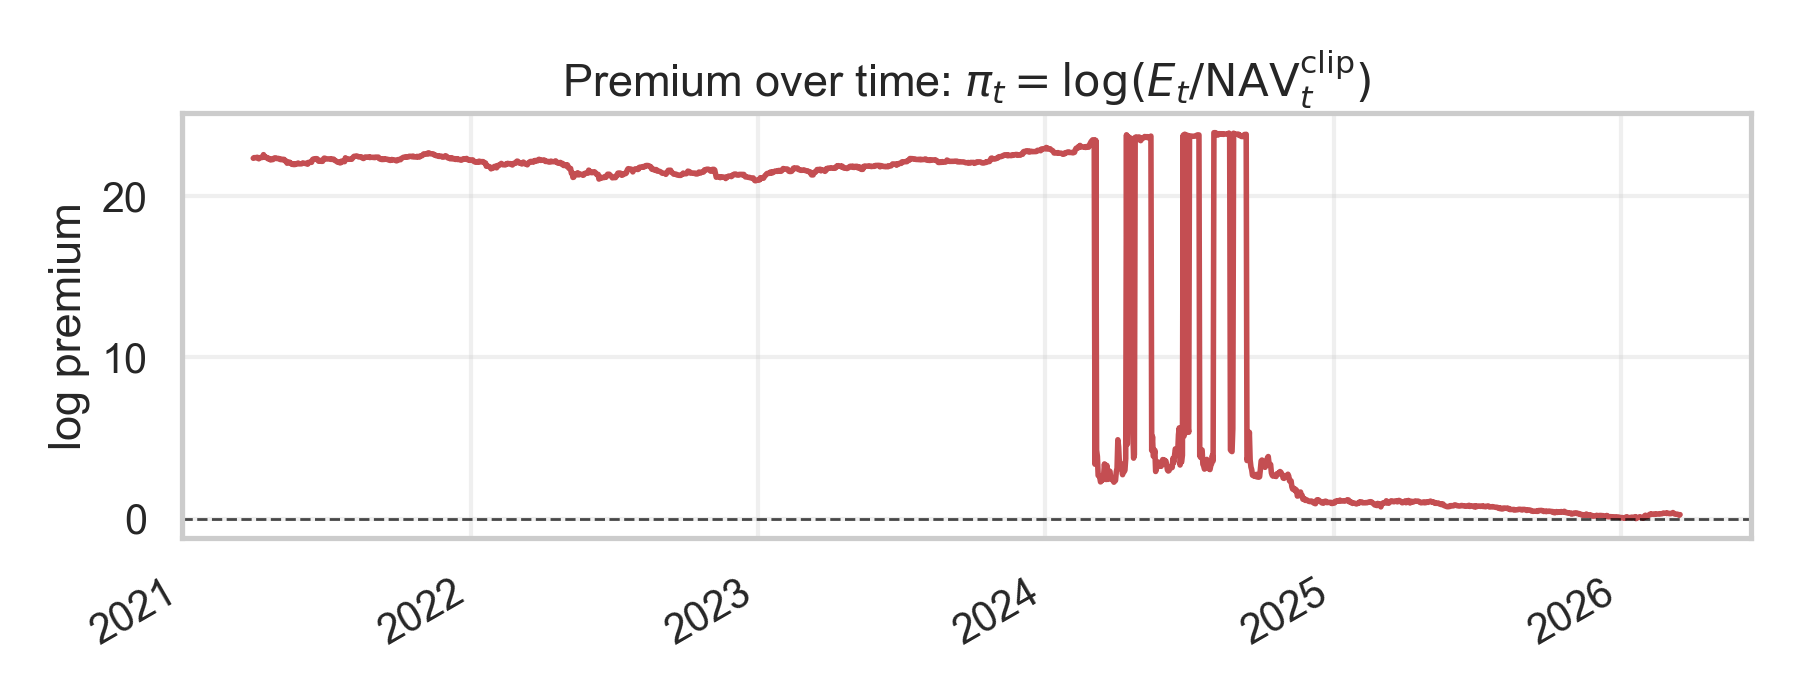
\includegraphics[width=0.85\textwidth]{../results/figures/premium_timeseries.png}
\caption{Historical log-premium $\pi_t = \log(E_t / \text{NAV}_t^{\text{clip}})$. The dashed line indicates the OU long-run mean $\theta = 0.705$. The premium exhibits clear mean-reverting behavior around this level.}
\label{fig:premium}
\end{figure}

\begin{figure}[H]
\centering
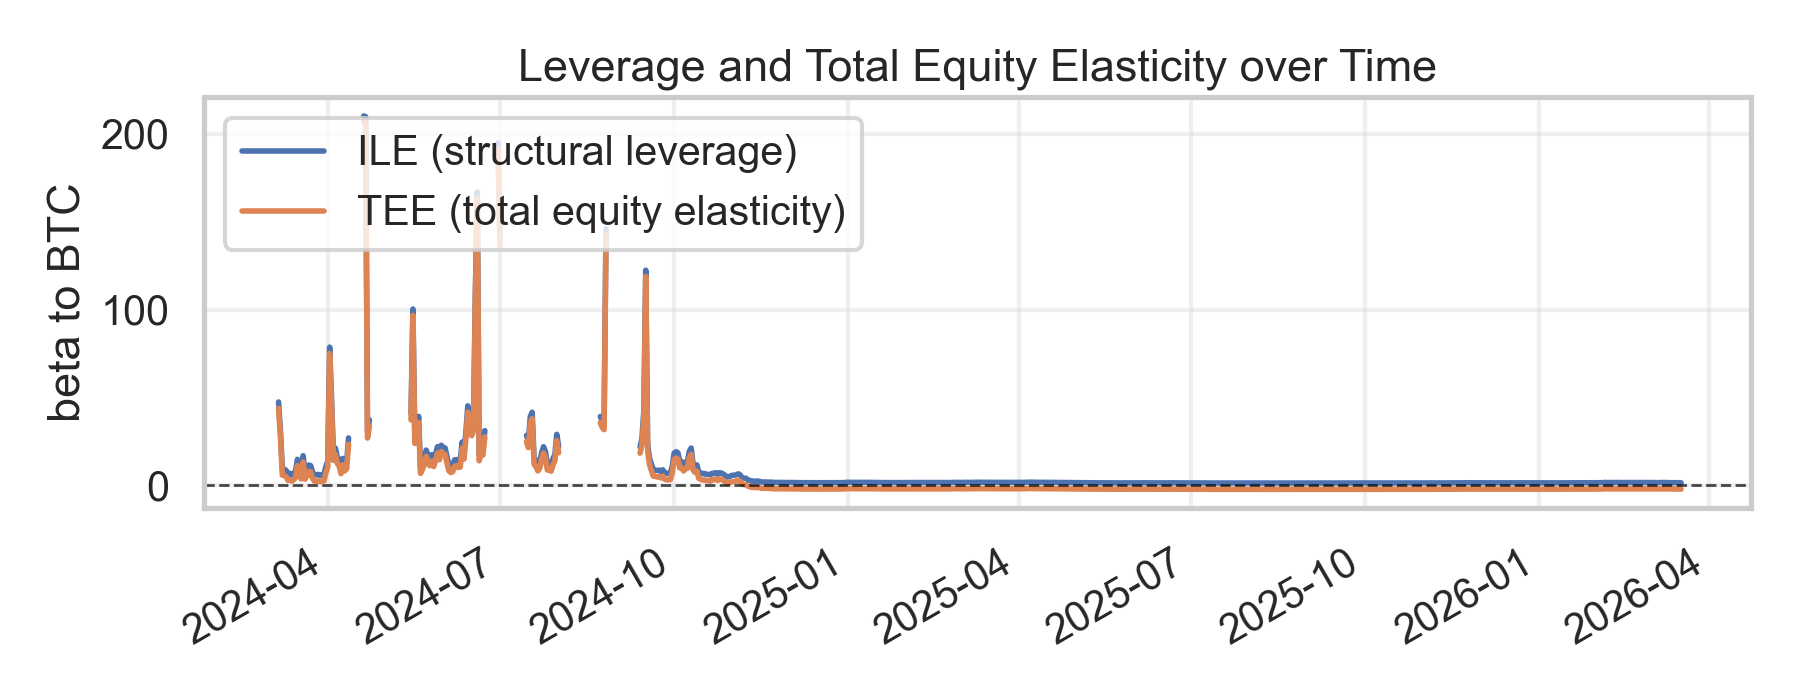
\includegraphics[width=0.85\textwidth]{../results/figures/ile_tee_timeseries.png}
\caption{Time series of Implied Leverage Elasticity (ILE) and Total Equity Elasticity (TEE). ILE has declined as BTC appreciation outpaced debt growth. TEE reflects the net of ILE and the negative premium--BTC sensitivity.}
\label{fig:ile_tee}
\end{figure}

\begin{figure}[H]
\centering
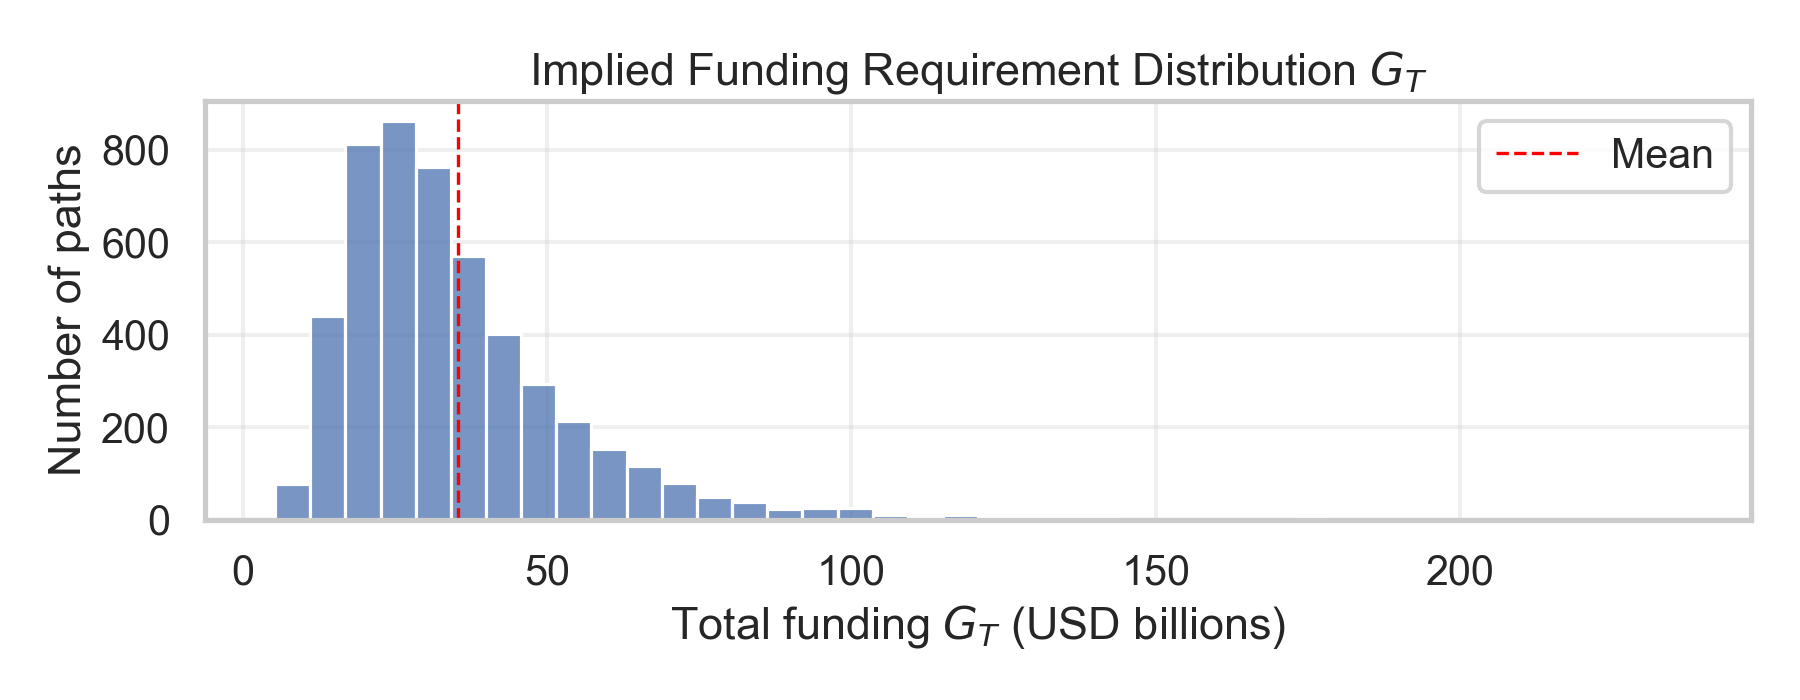
\includegraphics[width=0.85\textwidth]{../results/figures/ifrd_histogram.png}
\caption{Simulated three-year Implied Funding Requirement Distribution (IFRD). The distribution is right-skewed, with mean \$38.3B and 95th percentile \$80.3B.}
\label{fig:ifrd}
\end{figure}

\begin{figure}[H]
\centering
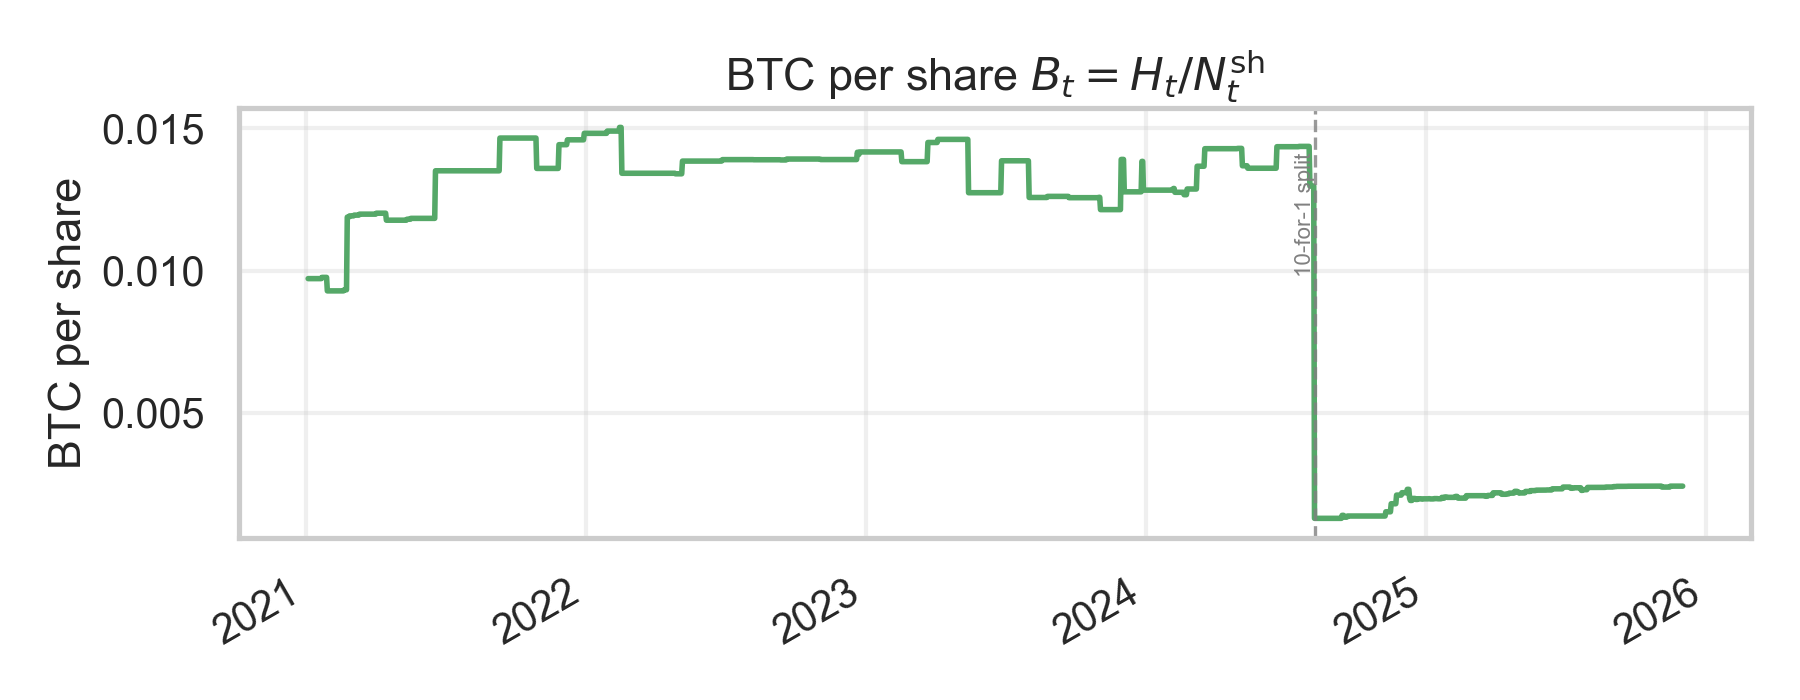
\includegraphics[width=0.85\textwidth]{../results/figures/btc_per_share_timeseries.png}
\caption{BTC per share ($B_t = H_t / N_t^{\text{sh}}$) over time. The upward trend confirms that Strategy's flywheel has been accretive despite significant share dilution.}
\label{fig:btc_per_share}
\end{figure}

\begin{figure}[H]
\centering
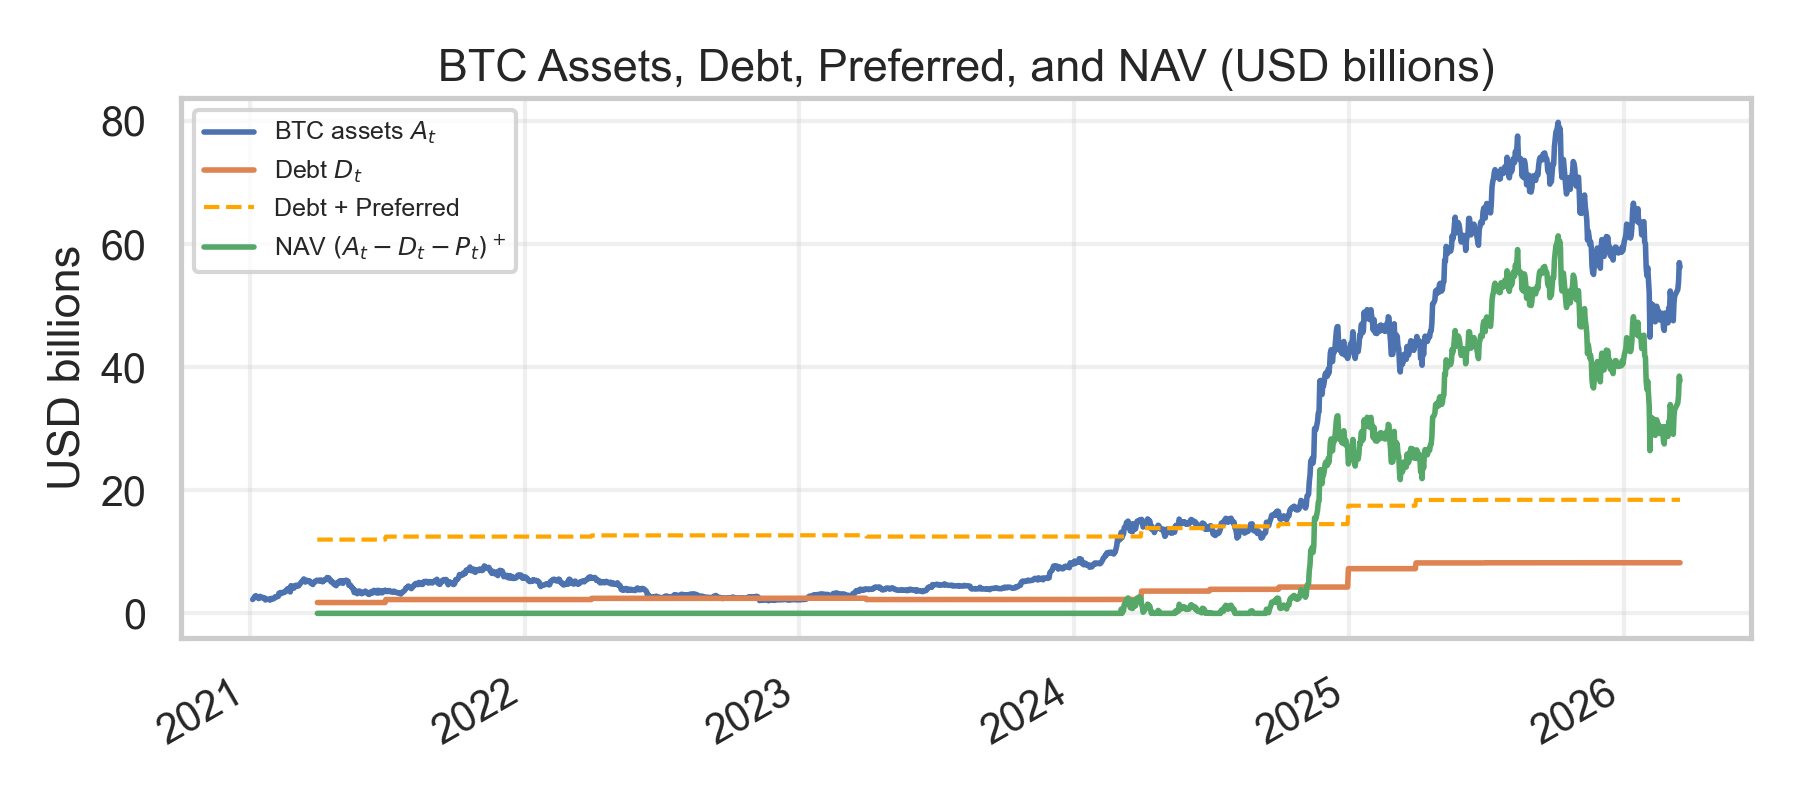
\includegraphics[width=0.85\textwidth]{../results/figures/assets_debt_nav.png}
\caption{BTC asset value ($A_t = H_t S_t$), outstanding debt ($D_t$), and NAV ($(A_t - D_t)^+$). The growing gap between assets and debt underpins the high survival probability.}
\label{fig:assets}
\end{figure}


\section{Discussion}
\label{sec:discussion}

\subsection{What the Model Tells Us About Strategy's Viability}

The calibrated model paints a picture of a company that has, through late 2025, successfully executed its leverage flywheel. Three findings stand out:

\textbf{First, the flywheel has been accretive.} The near-equality of total IBGR (18.3\%) and per-share IBGR (18.4\%) demonstrates that Strategy has acquired BTC at prices and share-issuance ratios that deliver increasing BTC per share. This is the core value proposition: common shareholders receive compounding exposure to BTC without directly purchasing it. The pure jump model ($\alpha = 0$) confirms that accretion occurs through discrete, large financing events rather than gradual accumulation---consistent with the company's pattern of multi-billion dollar ATM programs and convertible offerings.

\textbf{Second, balance-sheet leverage is currently modest.} An ILE of 1.17 means the equity's structural exposure to BTC barely exceeds 1:1. The 2020--2022 period saw much higher leverage (when BTC prices were lower relative to debt), but BTC appreciation has dramatically delevered the balance sheet. The \$8.2 billion debt stack is a small fraction of the \$56.1 billion BTC portfolio, providing substantial cushion. The 99.4\% three-year survival probability reflects this buffer.

\textbf{Third, the premium is currently depressed.} The PMRI of $-1.51$ suggests the market is pricing Strategy conservatively relative to the model's long-run equilibrium. Under the calibrated OU dynamics (half-life of $\sim$62 trading days), the premium is expected to mean-revert upward. Whether this represents a buying opportunity depends on whether the OU calibration (fitted primarily to the 2020--2025 sample) remains valid as the capital structure evolves with new preferred layers.

\subsection{Implications for Other BTC Treasury Companies}

Strategy's success has spawned imitators: several companies have adopted or announced Bitcoin treasury strategies, and the analytical framework developed here applies directly. The model's key inputs---BTC holdings, debt schedule, share count, and premium---are publicly observable for any such company, enabling cross-sectional comparison of flywheel efficiency and structural health.

The indicators have natural comparative interpretations. A company with high ILE and high IBGR is aggressively but accretively leveraging BTC. A company with high ILE but low or negative per-share IBGR is diluting shareholders without sufficient BTC accumulation. The PMRI can identify relative value across BTC treasury vehicles by comparing each company's premium deviation from its own long-run mean.

\subsection{Model Limitations}

Several limitations warrant discussion:

\textbf{Stationarity of the OU premium.} The OU specification assumes a constant long-run mean $\theta$ and mean-reversion speed $\kappa$. In practice, $\theta$ may shift as the BTC treasury model becomes better understood (or as new competitors enter), and $\kappa$ may vary with market microstructure and investor base composition. A regime-switching extension would address this but at the cost of additional parameters.

\textbf{Exogenous debt.} Modeling debt as deterministic ignores the strategic timing of issuance and the option value of convertible bonds. In reality, management times debt issuance opportunistically (issuing when premia are high and credit markets receptive), creating endogeneity that our model does not capture. A fuller model would make debt issuance intensity depend on the premium and BTC price, mirroring the holding dynamics.

\textbf{Risk-neutral vs.\ physical measure.} All indicators are computed under the physical measure, appropriate for real-world risk assessment. However, for pricing derivatives on MSTR equity or for risk-neutral valuation of the convertible bonds, a measure change would be needed, requiring specification of market prices of risk for both BTC and premium factors.

\textbf{Sample period.} The calibration uses data from 2020--2025, a period of generally favorable conditions for both BTC and the treasury model. Parameters estimated from this sample (particularly $\mu_S$ and $\theta$) may overstate the attractiveness of the strategy in a more adverse macro environment.

\textbf{Correlation stability.} The negative $\rho$ and $\gamma_{\pi S}$ are estimated as constants, but the relationship between BTC returns and the premium may be state-dependent---for instance, the premium may become more sensitive to BTC in high-leverage states or during market stress.

\subsection{Preferred Stock Extensions}

Strategy's capital stack has expanded significantly with the introduction of perpetual preferred stock series. Extending the model to accommodate these layers requires:

\textbf{Priority waterfall.} In liquidation and for dividend distribution, the capital stack follows: senior debt $\to$ convertible bonds $\to$ preferred stock (by seniority) $\to$ common equity. NAV must be allocated through this waterfall, with each tranche receiving its claim before the residual passes to the next.

\textbf{Perpetual dividend obligations.} Unlike debt maturities, preferred stock carries perpetual fixed dividends (8\% for STRK, 10\% for STRF). These create ongoing cash flow demands that affect the survival analysis---distress is no longer solely an asset-vs-debt question but includes the ability to service dividend obligations from BTC sales or new issuance.

\textbf{Conversion optionality.} STRK's convertibility into MSTR common stock at a fixed ratio (0.1 shares per STRK share) creates an embedded option that affects both the preferred valuation and the share count dynamics. When MSTR trades above the implied conversion price, STRK holders have an incentive to convert, diluting common equity but reducing preferred dividend obligations.

Incorporating these features into the simulation engine is a natural next step. The framework developed here---with its joint evolution of BTC price, premium, holdings, and share count---provides the scaffolding; what remains is to layer the priority waterfall on top of the existing NAV computation and add dividend cash-flow accounting to the survival analysis.

\subsection{Broader Implications for Corporate Finance}

The Bitcoin treasury vehicle represents a novel corporate form that challenges traditional frameworks. It is not a holding company (it actively trades), not a fund (it uses leverage and issues preferred equity), and not a traditional operating company (its ``operations'' are financial engineering). The structural model developed here suggests that this form can be viable---with 99\%+ survival probabilities---when operated with discipline (moderate leverage, accretive issuance). The key risk is not BTC volatility per se, but the potential for the flywheel to become \emph{dilutive}: if management issues shares or converts at unfavorable ratios, per-share BTC declines, the premium collapses, and the flywheel reverses. Our indicators---particularly the per-share IBGR and the PMRI---are designed to detect this transition early.


\section{Conclusion}
\label{sec:conclusion}

This paper develops a stochastic structural framework for valuing Bitcoin treasury vehicles---publicly traded companies whose primary asset is BTC, acquired through a leverage flywheel of equity, debt, and preferred stock issuance. We jointly model BTC price dynamics, the equity-over-NAV premium as an Ornstein--Uhlenbeck process, BTC holding accumulation as a compound Poisson process linked to the flywheel, and share-count evolution from issuance and conversion.

From this framework we derive five diagnostic indicators: the Implied BTC Growth Rate (IBGR), Implied Leverage Elasticity (ILE), Total Equity Elasticity (TEE), Premium Mean-Reversion Index (PMRI), and Implied Funding Requirement Distribution (IFRD). Together, these indicators decompose the valuation of a BTC treasury vehicle into its structural components---balance-sheet leverage, sentiment premium, accretion efficiency, and financing sustainability---providing investors and analysts with a rigorous toolkit for assessing these novel entities.

Calibrating to Strategy (MSTR) through December 2025, we find that the flywheel has been highly accretive (18.3\% annualized BTC growth, nearly identical per-share), balance-sheet leverage is currently moderate (ILE = 1.17), and the capital structure supports a three-year survival probability exceeding 99.4\%. The premium currently sits 1.5 standard deviations below its long-run mean, suggesting potential for mean-reversion.

These results are conditioned on the calibration sample and the model's assumptions of parameter stationarity. As Strategy's capital structure continues to evolve---with multiple preferred stock series, expanding ATM programs, and potential international vehicles---the framework presented here provides a foundation for increasingly granular analysis. The extension to multi-layer preferred capital stacks, outlined in the discussion, is a natural and important direction for future work.


\bibliographystyle{plainnat}
\bibliography{references}

\end{document}
